\documentclass[11pt]{article}

% --------------------
% Packages
% --------------------
\usepackage[margin=1in]{geometry}
\usepackage{amsmath, amssymb, amsfonts}
\usepackage{graphicx}
\usepackage{float}
\usepackage{caption}
\usepackage{booktabs}
\usepackage{enumitem}
\usepackage{mathtools}
\usepackage{hyperref}
\usepackage{helvet}
\usepackage{titlesec}
\usepackage{titling}
\renewcommand{\familydefault}{\sfdefault}

\titleformat*{\subsection}{\fontsize{11}{15.6}\selectfont\bfseries}
\setlength{\parindent}{0in}

% --------------------
% Formatting
% --------------------
\setlength{\droptitle}{-1.75cm}
\title{Numerical PDEs Homework \#4}
\author{Hope Elsayed}
\date{} % Leaves the date blank
\begin{document}

\maketitle
\vspace{-1.5cm}

% ==================================================
\section*{Allen-Cahn Equation - Setup}
% ==================================================

Consider the two-dimensional Allen-Cahn equation
\[
    \phi_t = \epsilon^2 \nabla^2 \phi - F'(\phi),
    \qquad (x,y) \in \Omega = [0,1]\times[0,1],
\]
where
\[
    F(\phi) = \frac{(\phi^2-1)^2}{4},
    \qquad
    F'(\phi) = \phi^3-\phi.
\]

Therefore, the Allen-Cahn equation can also be written as
\[
    \phi_t = \epsilon^2 \nabla^2 \phi + \phi-\phi^3.
\]

The function $\phi(x,y,t)$ describes the phase of two  immiscible fluids. The values $\phi=-1$ and $\phi=1$ represent the two distinct phases, such as oil and water, while values between $-1$ and $1$ represent the transition region between  the phases. The parameter $\epsilon$ controls the width of this interface. \\

Homogeneous Neumann boundary conditions are imposed on 
all four boundaries:
\begin{align*}
    \phi_x(0,y,t) &= \phi_x(1,y,t)=0,\\
    \phi_y(x,0,t) &= \phi_y(x,1,t)=0.
\end{align*}

The initial condition is generated using normally  distributed random values with variance $\epsilon^2$.  The mean is then subtracted so that the initial condition has zero mean.

\newpage

% ==================================================
\section*{Problem 1: Basic Operator Splitting}
% ==================================================

Implement a finite difference discretization of the Allen-Cahn equation using $\Delta x=\Delta y=\epsilon$. Generate a random initial condition with zero mean and simulate the solution until $t_{\mathrm{final}}=50$.

Integrate in time using an operator splitting scheme that separates the diffusion and reaction terms. Experiment with different time step sizes to determine an appropriate $\Delta t$. \\

\textbf{Solution: }

% --------------------------------------------------
\subsection*{Spatial Discretization}
% --------------------------------------------------

The domain was discretized using a uniform grid with $N_x=N_y=N=100$. The Laplacian was approximated using a centered five-point finite difference stencil. \\

Let $D$ denote the one-dimensional finite difference matrix for the second derivative with homogeneous Neumann boundary conditions. The two-dimensional Laplacian matrix was constructed using Kronecker products:
\[
    L=I_N\otimes D+D\otimes I_N.
\]

% --------------------------------------------------
\subsection*{Operator Splitting}
% --------------------------------------------------

The Allen-Cahn equation was separated into two equations:
\begin{align*}
    \phi_t &= \epsilon^2\nabla^2\phi
    &&\text{(Diffusion)},\\
    \phi_t &= \phi-\phi^3
    &&\text{(Reaction)}.
\end{align*}

At each time step, the diffusion equation is solved first, followed by the reaction equation using the result of the diffusion step as its initial condition.

\subsubsection*{Step 1: Diffusion}

The diffusion equation was discretized in time using Backward Euler:
\[
    \frac{\phi^*-\phi^n}{\Delta t}
    =\epsilon^2L\phi^*.
\]

Rearranging gives the linear system
\[
    \boxed{
        (I-\Delta t\epsilon^2L)\phi^*=\phi^n.
    }
\]

\subsubsection*{Step 2: Reaction}

The reaction equation is an ODE that can be solved analytically:
\[
    \frac{d\phi}{dt}=\phi-\phi^3,
    \qquad \phi(0)=\phi_0.
\]

Using Wolfram Alpha to solve this ODE, we obtain
\[
    \phi^{\mathrm{ODE}}(t,\phi_0)
    =
    \frac{\phi_0}
    {\sqrt{\phi_0^2+(1-\phi_0^2)e^{-2t}}}.
\]

Using $\phi^*$ from the diffusion step as the initial 
condition and evaluating at $t=\Delta t$, we obtain
\[
    \boxed{
    \phi^{n+1}
    =
    \frac{\phi^*}
    {\sqrt{(\phi^*)^2+
    (1-(\phi^*)^2)e^{-2\Delta t}}}.
    }
\]

% --------------------------------------------------
\subsection*{Numerical Solution}
% --------------------------------------------------
A fixed random seed was used so that the results 
were reproducible.

\begin{figure}[H]
    \centering
    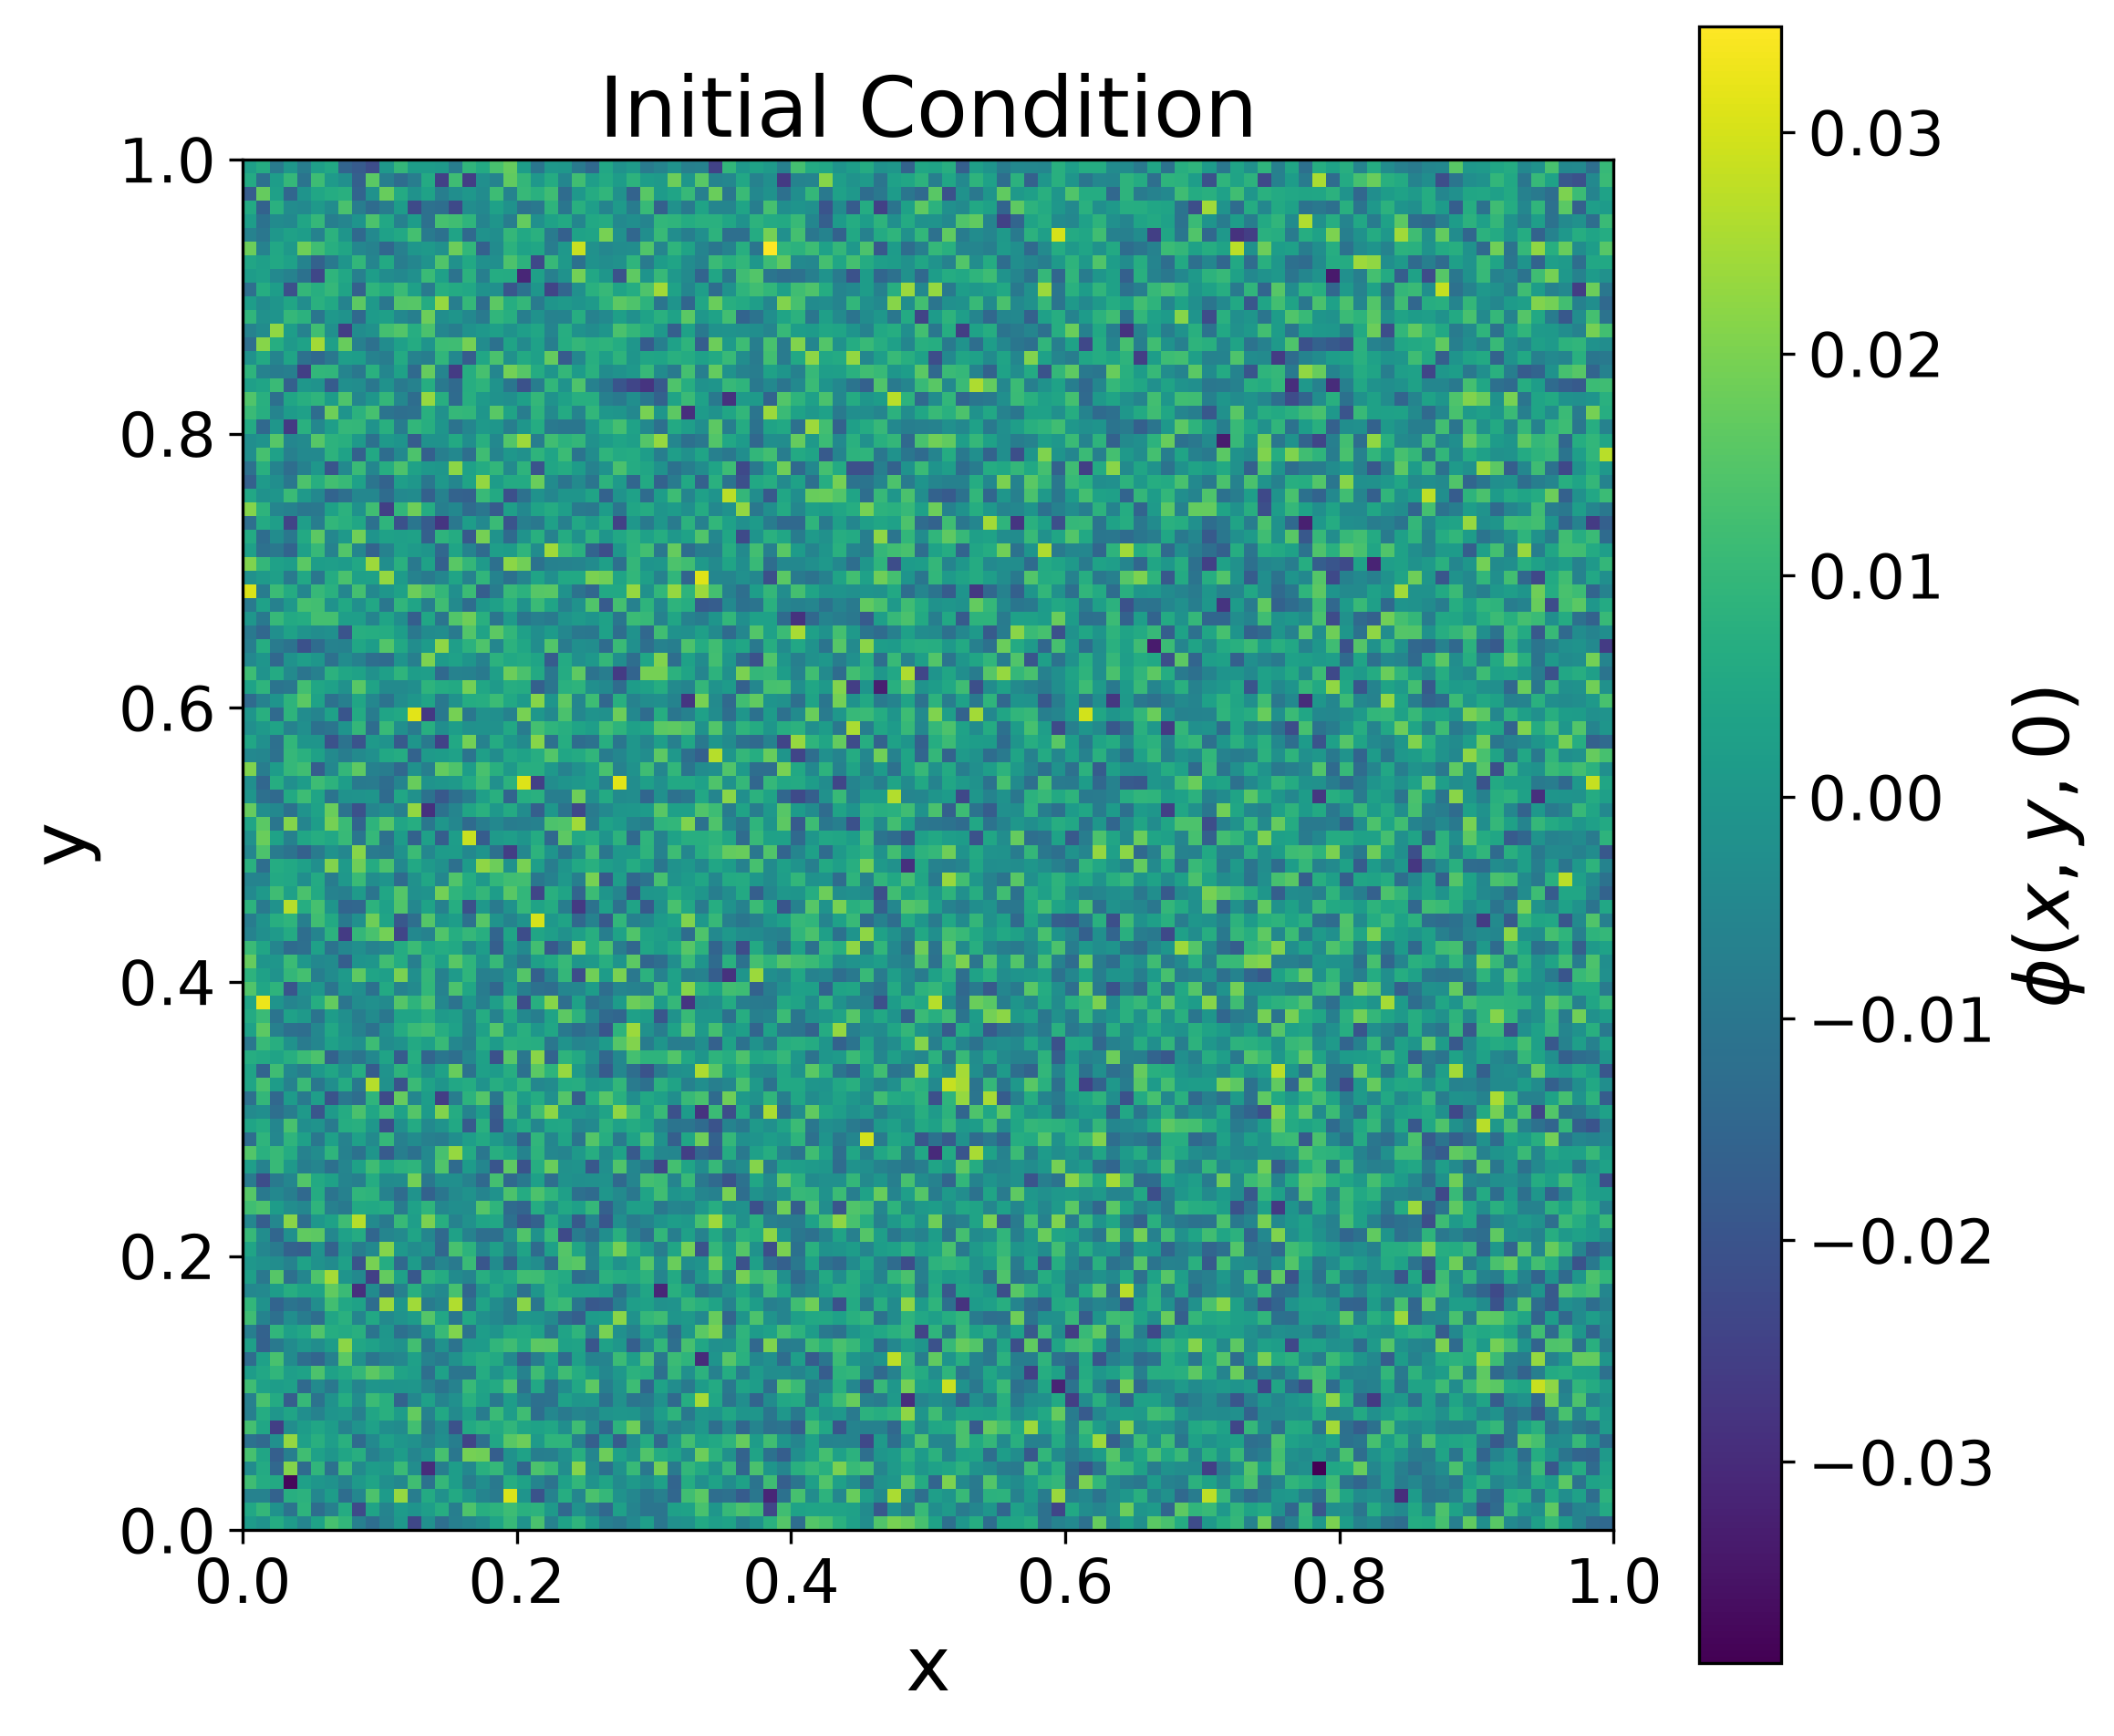
\includegraphics[width=0.75\textwidth]
    {initial_condition.png}
    \caption{Random initial condition with approximately 
    zero mean and $\epsilon=0.01$.}
    \label{fig:initial_condition}
\end{figure}

The Allen-Cahn equation was solved using $\Delta t=h=0.01$ until $t_{\mathrm{final}}=50$, requiring 5000 time steps.

\begin{figure}[H]
    \centering
    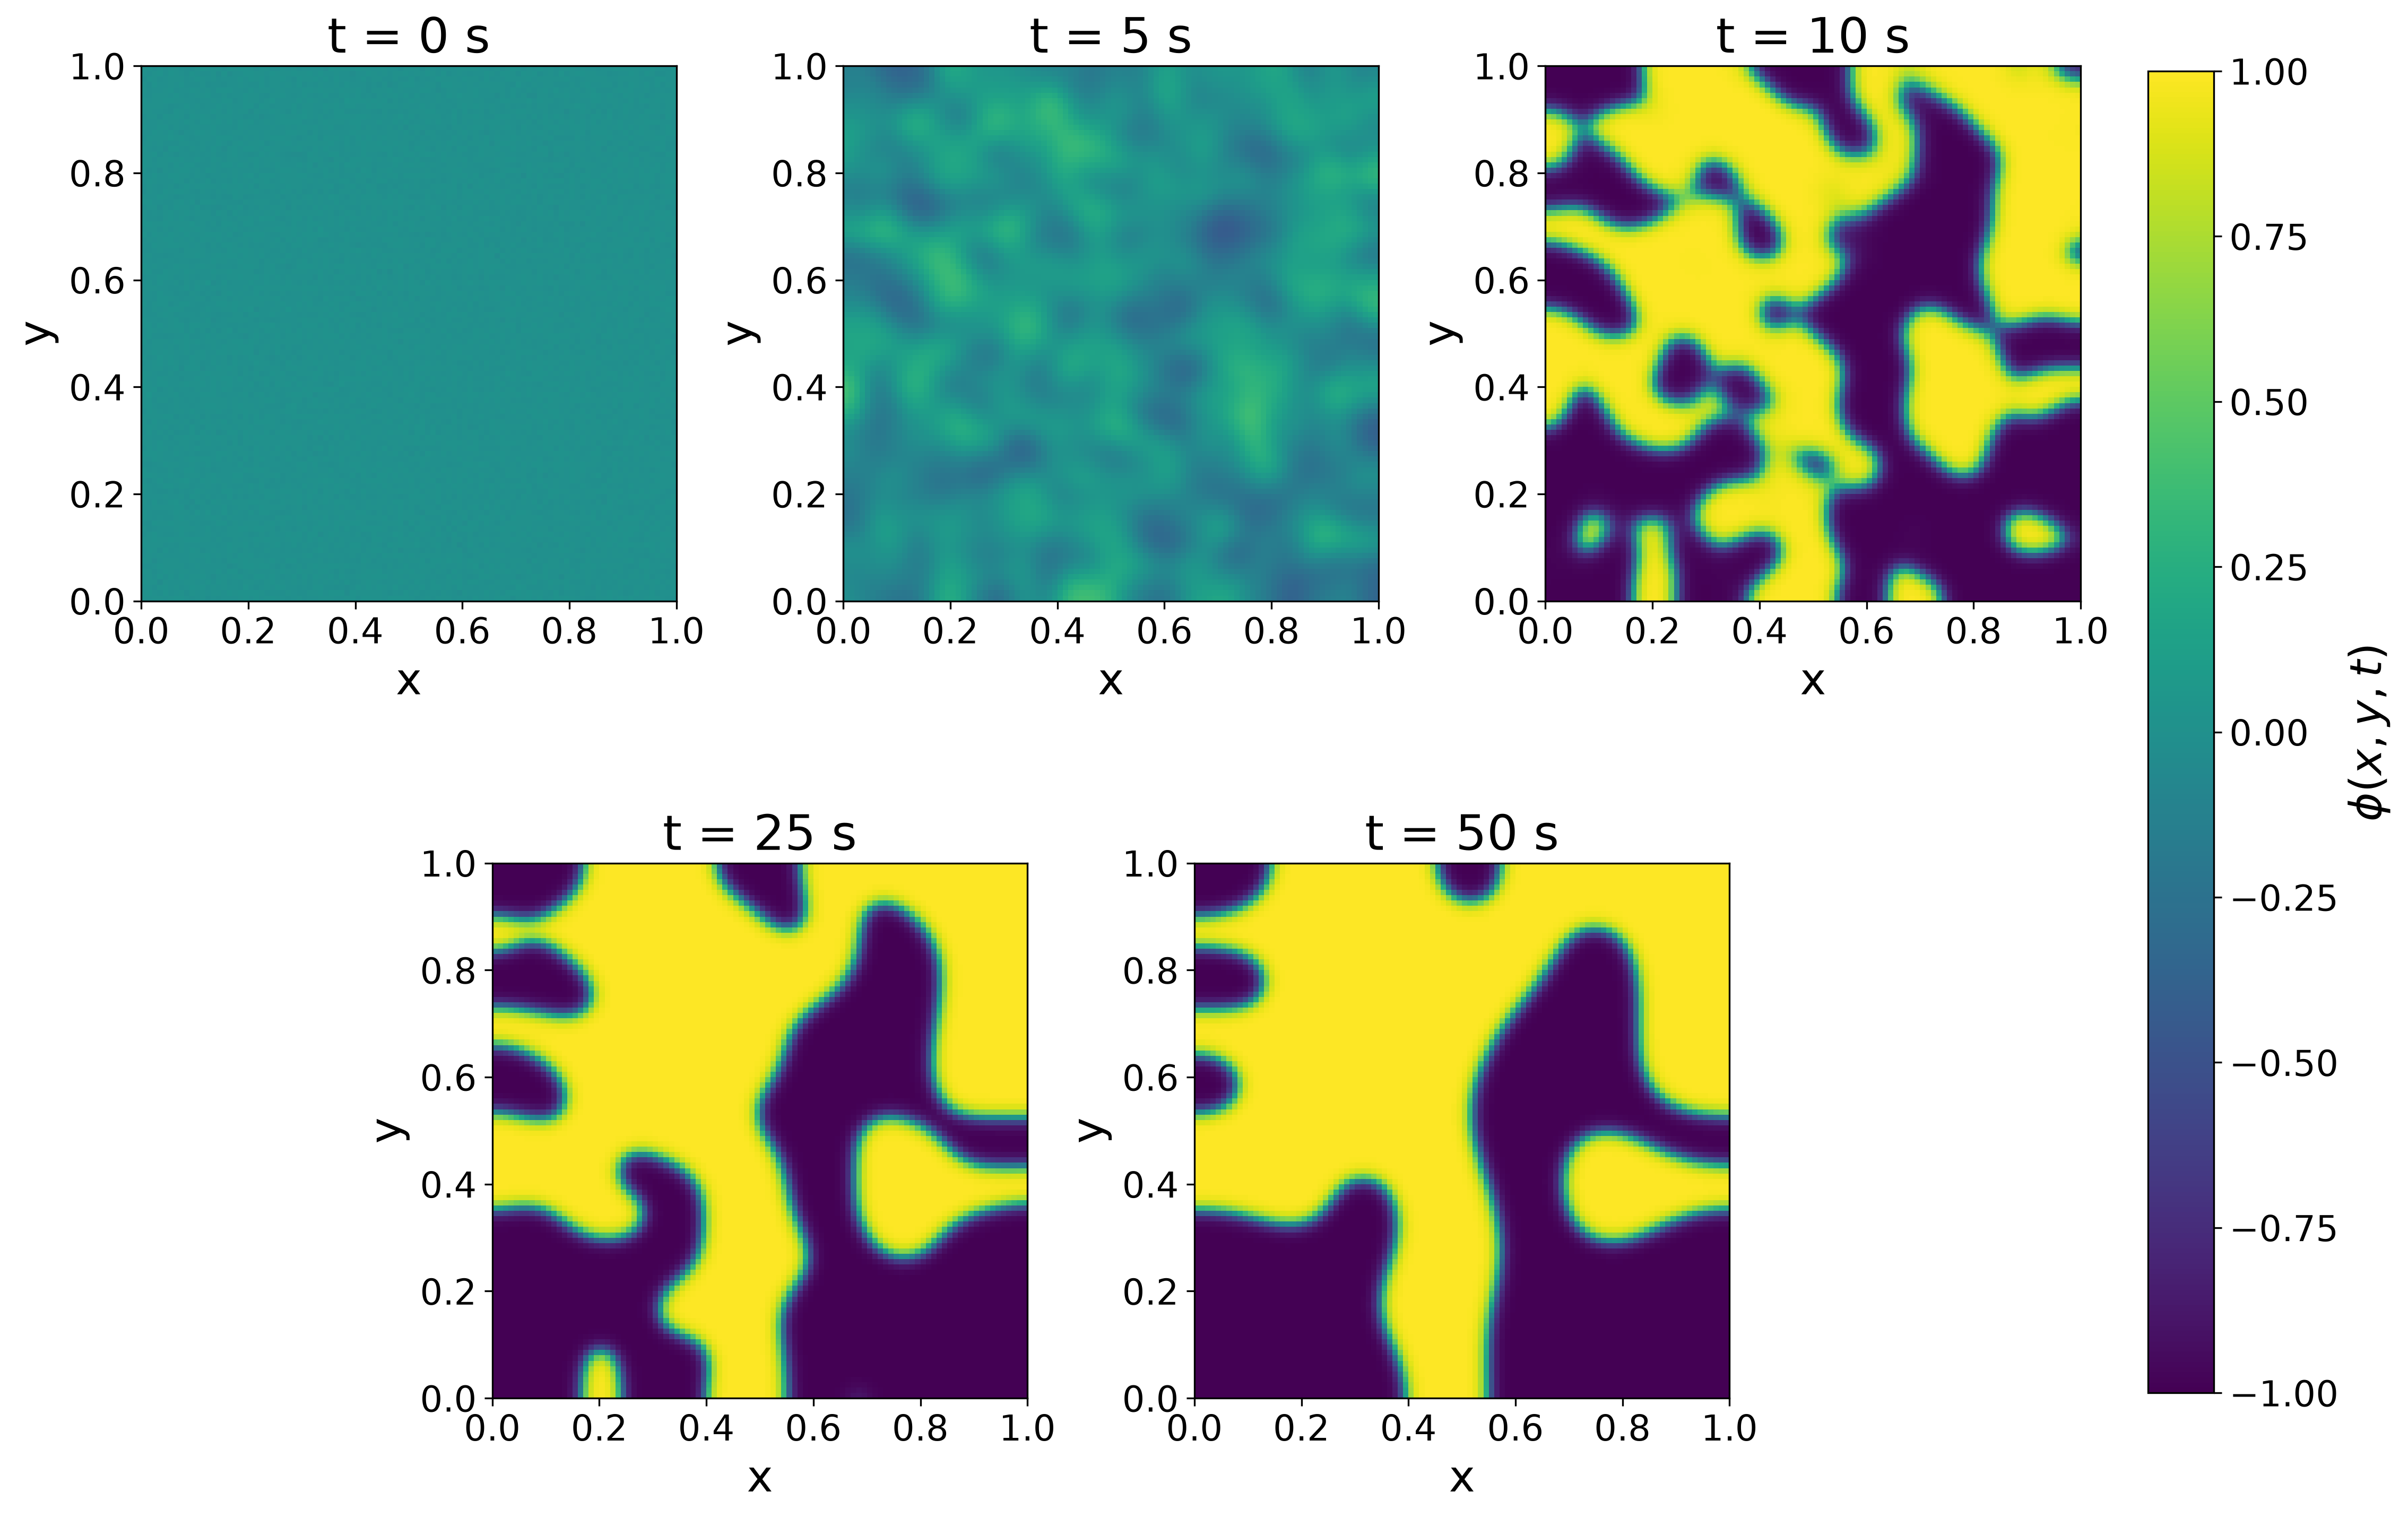
\includegraphics[width=\textwidth]
    {basic_snapshots.png}
    \caption{Numerical solution of the basic Allen-Cahn 
    equation at $t=0$, 5, 10, 25, and 50.}
    \label{fig:basic_snapshots}
\end{figure}

Figure~\ref{fig:basic_snapshots} shows that the initially well-mixed fluids begin separating into two distinct phases. Over time, the diffusion term smooths the randomness and the reaction term moves the solution toward $\phi=\pm1$. By $t=10$, the two phases are clearly distinguishable. At $t=50$, the minimum and maximum values of the numerical solution are approximately 
$-1$ and $1$, respectively.

% --------------------------------------------------
\subsection*{Time Step Experimentation}
% --------------------------------------------------
Backward Euler is unconditionally stable for the diffusion equation, meaning that we are not restricted to small time steps for the diffusion step. However, because we are solving the diffusion and reaction equations separately, we introduce additional error. \\

Even if the numerical solution remains between $-1$ and $1$, this does not necessarily mean that the solution is accurate. So, I wanted to experiment with different time step sizes to see how large of a time step I could use while still obtaining an accurate solution. \\

Although Backward Euler is unconditionally stable for the diffusion equation, this alone does not guarantee stability of the full nonlinear operator splitting scheme. However, the analytical reaction step preserves the interval $[-1,1]$, and the numerical solutions remained bounded for all of the time step sizes tested. \\

To investigate the effect of the time step size, 
I solved the Allen-Cahn equation using
\[
    \Delta t=0.01,\ 0.05,\ 0.10,\ \text{and }0.50.
\]

Because an exact solution to the full PDE is not available, a numerical reference solution was computed using a smaller time step of
\[
    \Delta t_{\mathrm{ref}}=0.005.
\]

The relative $L_2$ error at $t=50$ was calculated as
\[
    \mathrm{err}_{\phi}
    =
    \frac{
        \|\phi_{\Delta t}-\phi_{\mathrm{ref}}\|_2
    }{
        \|\phi_{\mathrm{ref}}\|_2
    }.
\]

\begin{figure}[H]
    \centering
    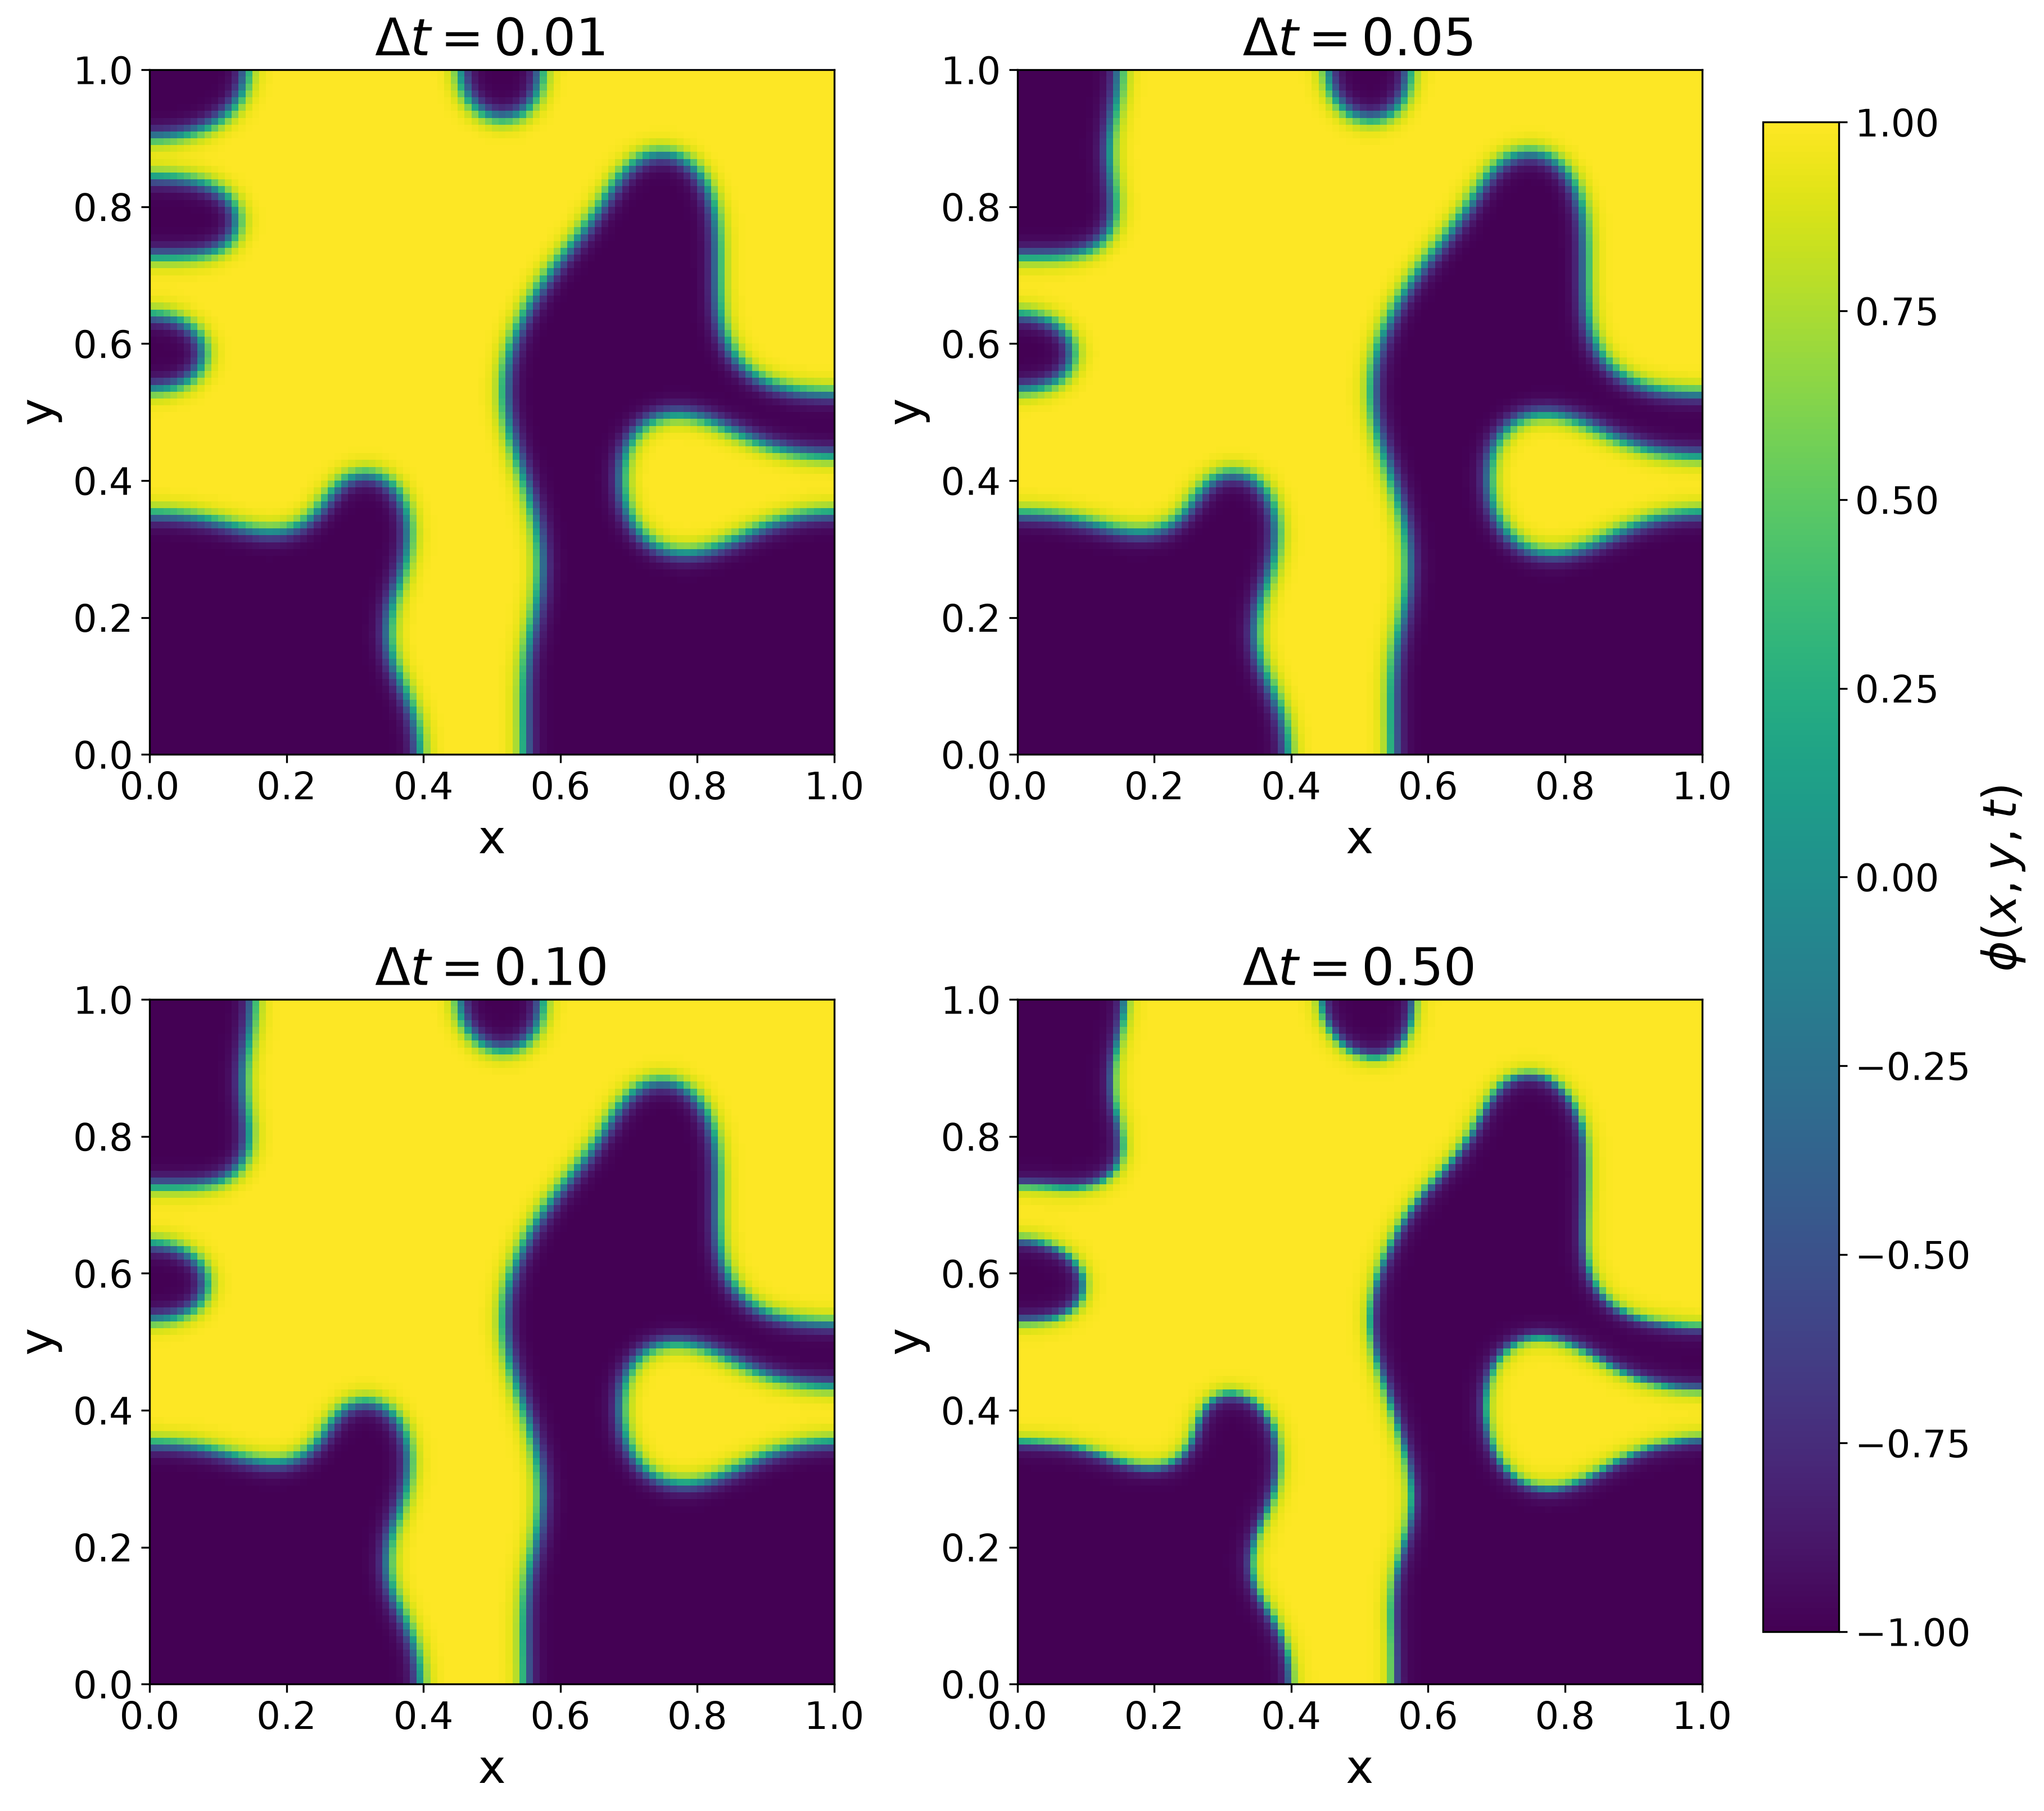
\includegraphics[width=\textwidth]
    {timestep_comparison.png}
    \caption{Numerical solutions of the basic Allen-Cahn 
    equation at $t=50$ for different time step sizes.}
    \label{fig:timestep_comparison}
\end{figure}

Figure~\ref{fig:timestep_comparison} shows that the solutions have similar overall phase distributions. However, the two negative-phase regions in the upper-left corner merge when larger time steps are used. There are also smaller differences in the locations of the interfaces.

\begin{table}[H]
    \centering
    \caption{Relative errors and computational times 
    for different time step sizes.}
    \label{tab:timestep}
    \begin{tabular}{|c|c|c|c|}
        \hline
        $\Delta t$ & Time Steps & Relative Error 
        & Runtime (s) \\ [0.5ex]
        \hline
        0.01 & 5000 & $4.2891\times10^{-3}$ & 6.67\\
        0.05 & 1000 & $2.0896\times10^{-1}$ & 1.50\\
        0.10 & 500  & $2.1635\times10^{-1}$ & 0.72\\
        0.50 & 100  & $2.7082\times10^{-1}$ & 0.14\\
        \hline
    \end{tabular}
\end{table}

\begin{figure}[H]
    \centering
    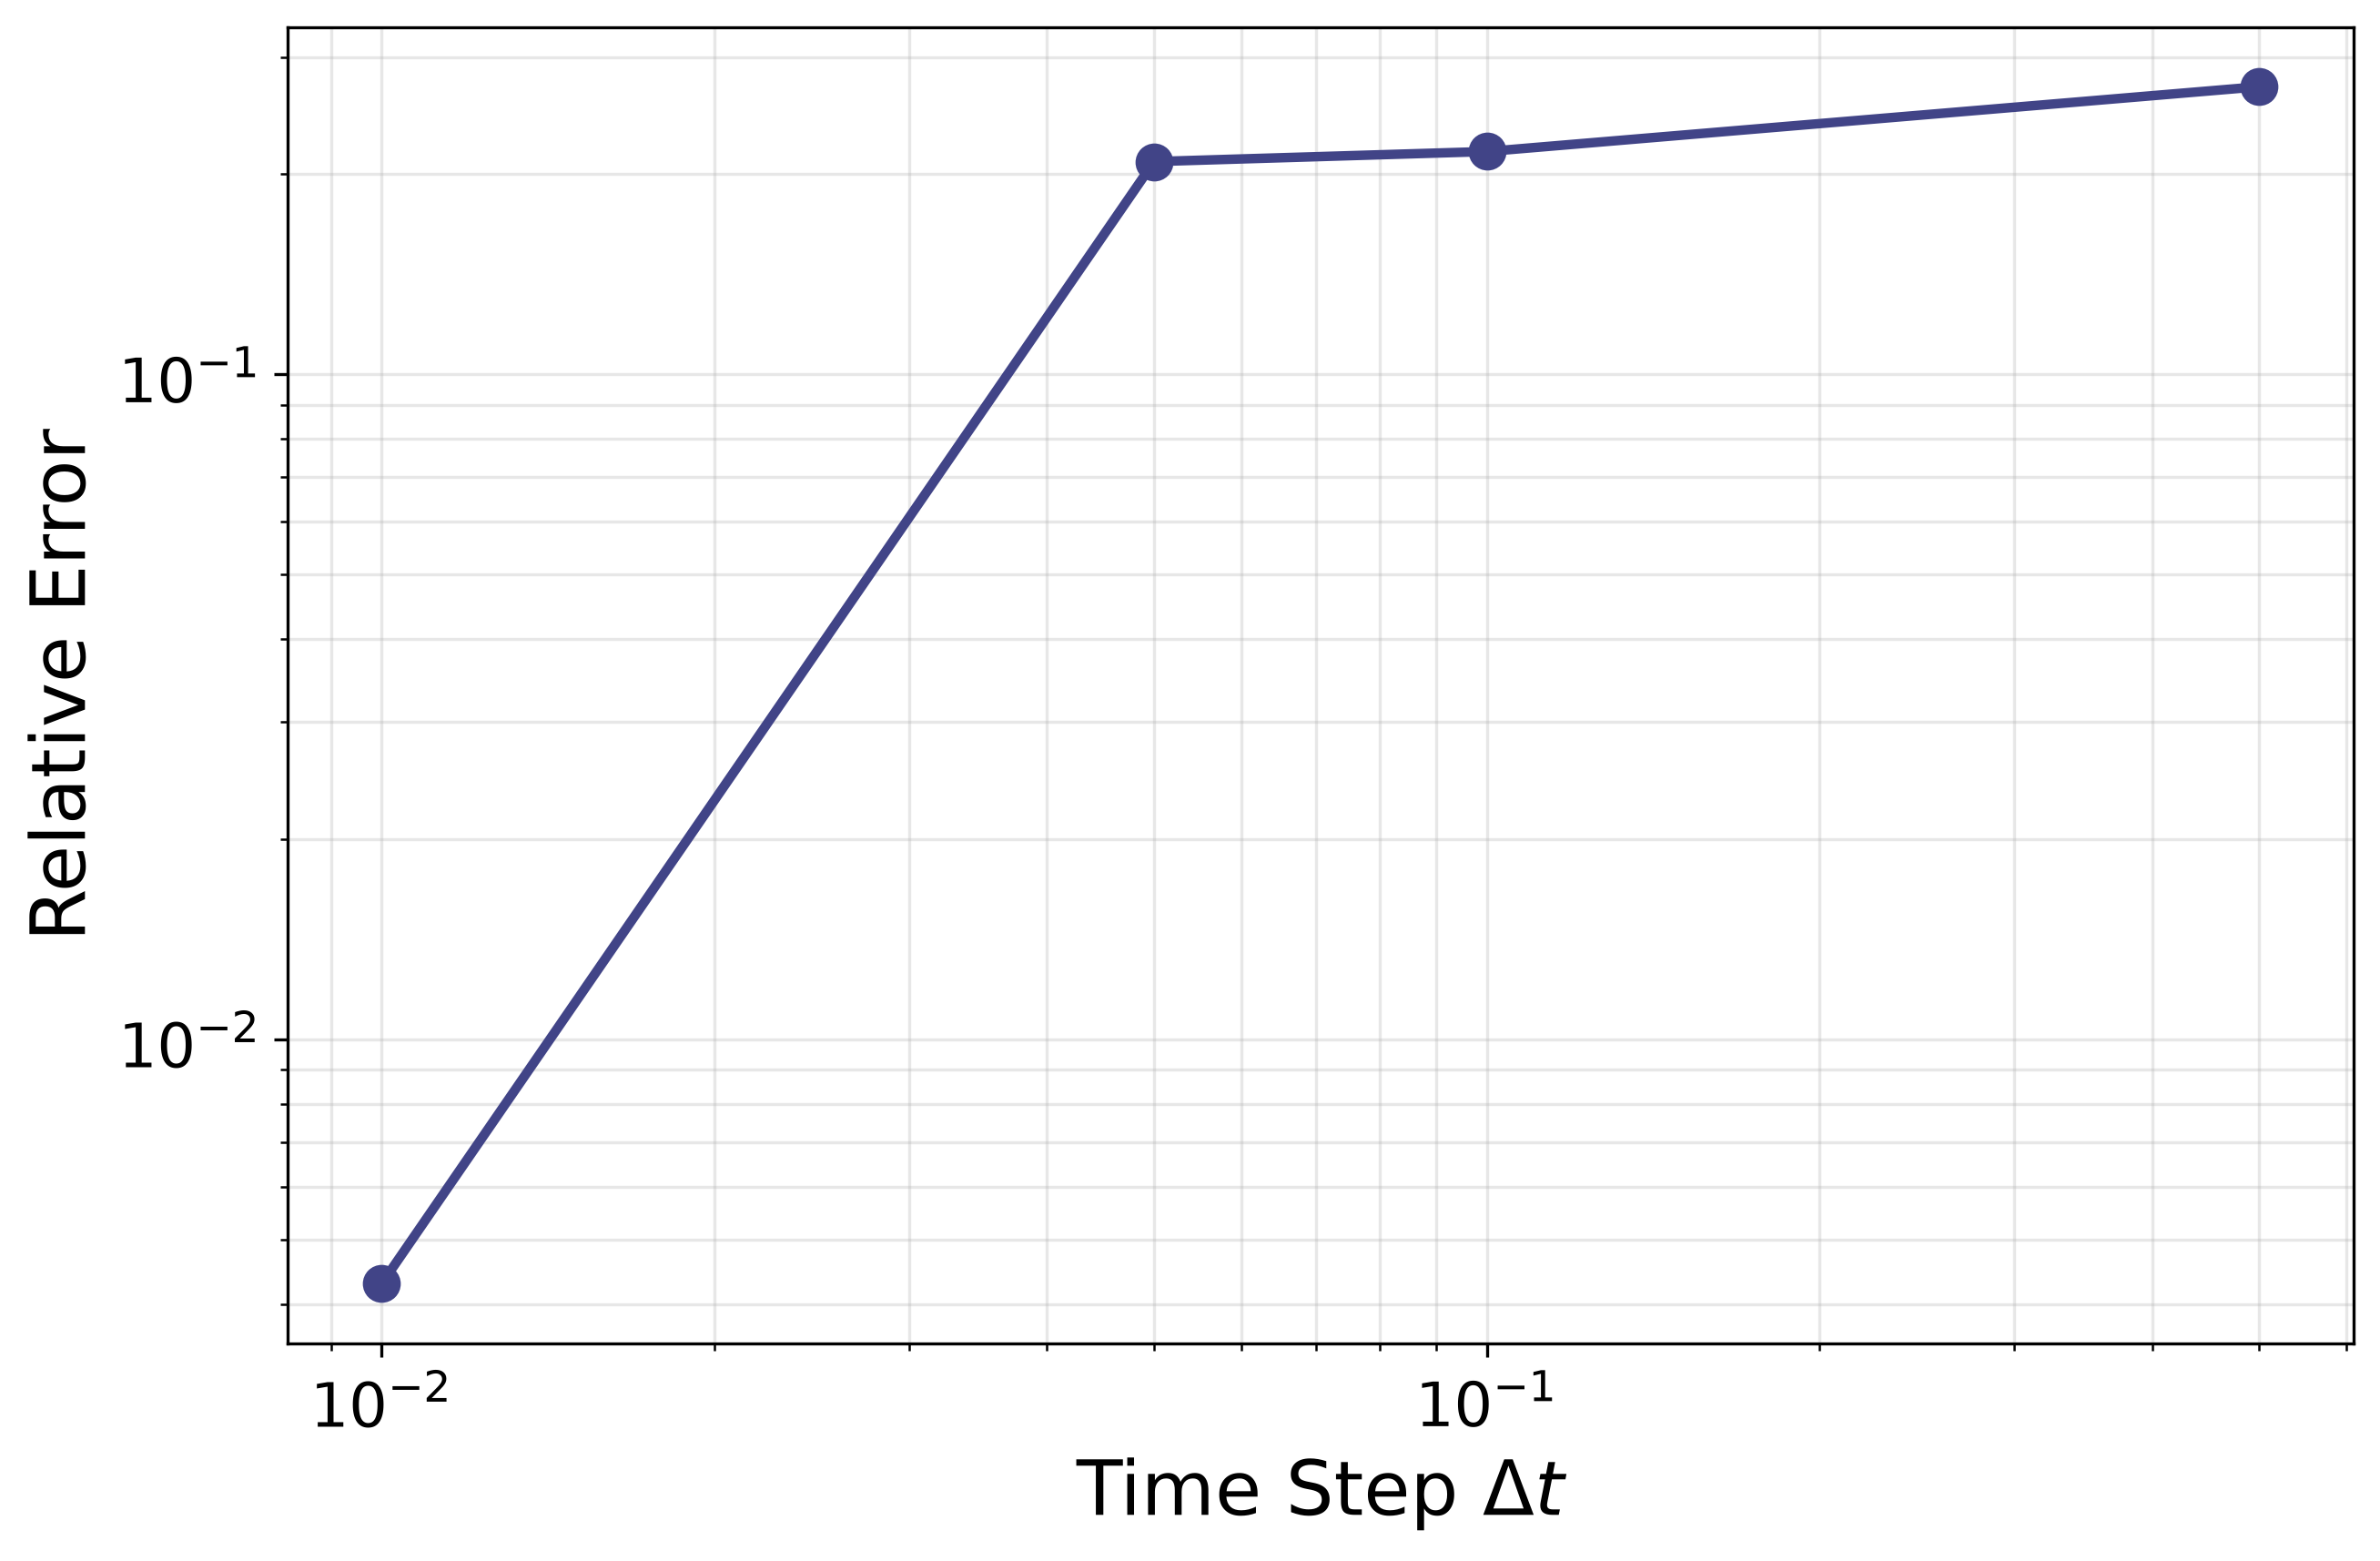
\includegraphics[width=\textwidth]
    {timestep_error.png}
    \caption{Relative $L_2$ error at $t=50$ for 
    increasing time step sizes compared with the 
    reference solution.}
    \label{fig:timestep_error}
\end{figure}

Figure~\ref{fig:timestep_error} and Table~\ref{tab:timestep} show that the relative error increases as the time step size increases. In particular, increasing $\Delta t$ from 0.01 to 0.05 increases the relative error from approximately 0.43\% to 20.90\%. This large increase in time step size can be visually observed in the numerical solution in Figure~\ref{fig:timestep_comparison}. \\

Overall, the larger time steps produced less accurate solutions. Therefore, I chose to continue using $\Delta t=0.01$ because it produced a small relative error and didn't take long to run.

% --------------------------------------------------
\subsection*{Total Mass}
% --------------------------------------------------
The total mass of the system is defined as
\[
    M(t)=\int_\Omega\phi(x,y,t)\,dx\,dy.
\]

The discrete approximation of the total mass is
\[
    M^n=h^2\sum_{i,j}\phi_{ij}^n.
\]

\begin{figure}[H]
    \centering
    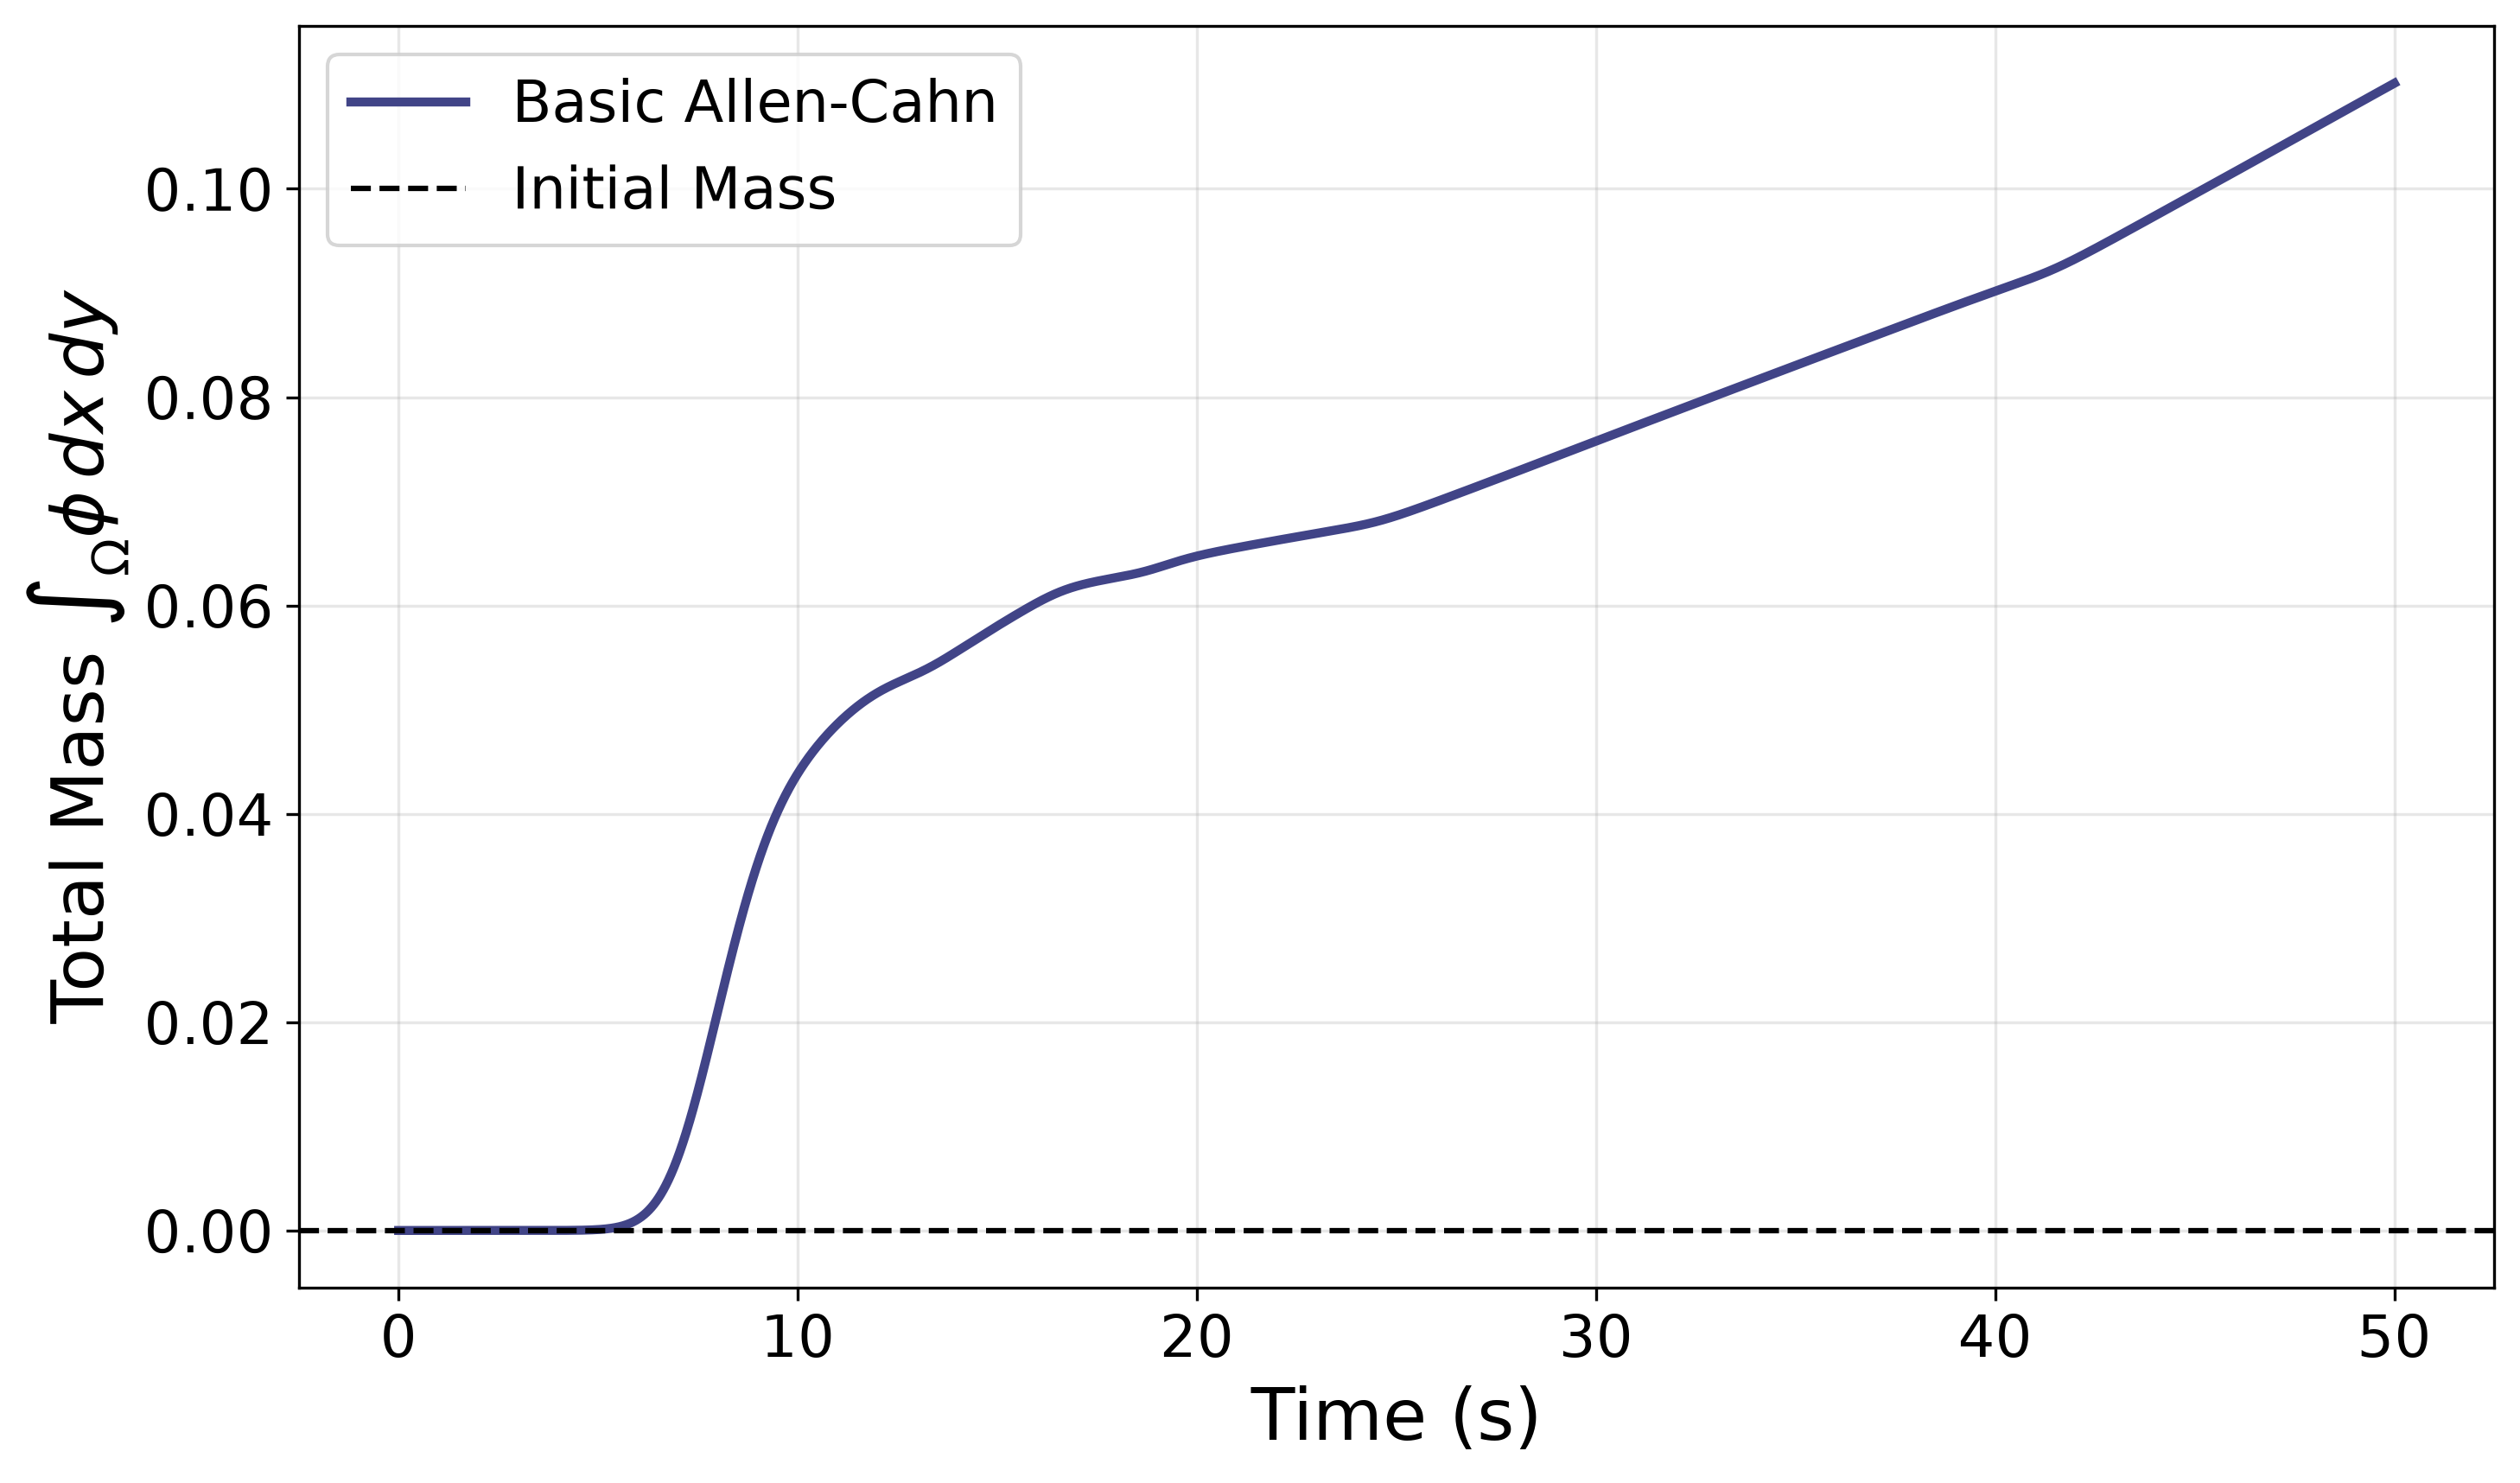
\includegraphics[width=\textwidth]
    {basic_mass.png}
    \caption{Total mass over time for the basic 
    Allen-Cahn equation.}
    \label{fig:basic_mass}
\end{figure}

Figure~\ref{fig:basic_mass} shows that the total mass is not conserved. The initial mass was approximately zero, but the final mass at $t=50$ was
\[
    M(50)=0.1101278.
\]

\newpage

% ==================================================
\section*{Problem 2: Conservative Allen-Cahn}
% ==================================================

Modify the Allen-Cahn equation so that the total mass of the system is conserved. Consider the modified equation
\[
    \phi_t=
    \epsilon^2\nabla^2\phi-F'(\phi)
    +\beta(t)\sqrt{F(\phi)},
\]
where
\[
    \beta(t)=
    \frac{
        \displaystyle\int_\Omega F'(\phi)\,dx\,dy
    }{
        \displaystyle\int_\Omega\sqrt{F(\phi)}\,dx\,dy
    }.
\]

Show that this modified equation conserves the total  mass. Then modify the operator splitting scheme from Problem 1 by introducing a discrete mass correction step. Derive the discrete correction coefficient $\beta^{n+1}$ and demonstrate numerically that the modified equation conserves mass. \\

\textbf{Solution: } 

% --------------------------------------------------
\subsection*{Continuous Mass Conservation}
% --------------------------------------------------

The total mass is defined as
\[
    M(t)=\int_\Omega\phi(x,y,t)\,dx\,dy.
\]

Differentiating with respect to time gives
\begin{align*}
    \frac{dM}{dt}
    &=\int_\Omega\phi_t\,dx\,dy.
\end{align*}

For the basic Allen-Cahn equation,
\[
    \frac{dM}{dt}
    =
    \epsilon^2\int_\Omega\nabla^2\phi\,dx\,dy
    -\int_\Omega F'(\phi)\,dx\,dy.
\]

Using the divergence theorem,
\begin{align*}
    \int_\Omega\nabla^2\phi\,dx\,dy
    &=
    \int_{\partial\Omega}\nabla\phi\cdot\mathbf{n}\,ds\\
    &=
    \int_{\partial\Omega}
    \frac{\partial\phi}{\partial n}\,ds\\
    &=0,
\end{align*}
which follows from the homogeneous Neumann boundary conditions. \\

Therefore, for the basic Allen-Cahn equation,
\[
    \frac{dM}{dt}
    =-\int_\Omega F'(\phi)\,dx\,dy
    =\int_\Omega(\phi-\phi^3)\,dx\,dy.
\]

This integral is not necessarily zero, which explains why mass is not conserved in Problem 1. \\

For the conservative Allen-Cahn equation,
\begin{align*}
    \frac{dM}{dt}
    &=
    \epsilon^2\int_\Omega\nabla^2\phi\,dx\,dy
    -\int_\Omega F'(\phi)\,dx\,dy\\
    &\qquad
    +\beta(t)\int_\Omega\sqrt{F(\phi)}\,dx\,dy.
\end{align*}

Again, the diffusion term integrates to zero because 
of the homogeneous Neumann boundary conditions. 
Therefore,
\[
    \frac{dM}{dt}
    =
    -\int_\Omega F'(\phi)\,dx\,dy
    +\beta(t)\int_\Omega\sqrt{F(\phi)}\,dx\,dy.
\]

Substituting the given expression for $\beta(t)$,
\begin{align*}
    \frac{dM}{dt}
    &=
    -\int_\Omega F'(\phi)\,dx\,dy\\
    &\quad+
    \frac{
        \displaystyle\int_\Omega F'(\phi)\,dx\,dy
    }{
        \displaystyle\int_\Omega\sqrt{F(\phi)}\,dx\,dy
    }
    \int_\Omega\sqrt{F(\phi)}\,dx\,dy\\
    &=
    -\int_\Omega F'(\phi)\,dx\,dy
    +\int_\Omega F'(\phi)\,dx\,dy\\
    &=0.
\end{align*}

Thus, assuming the denominator in $\beta(t)$ is nonzero,
\[
    \boxed{
        \frac{dM}{dt}=0
        \qquad\Longrightarrow\qquad
        M(t)=M(0).
    }
\]

Therefore, the modified Allen-Cahn equation conserves the total mass of the system.

% --------------------------------------------------
\subsection*{Conservative Operator Splitting}
% --------------------------------------------------

The operator splitting scheme from Problem 1 was modified by adding a third step that corrects the mass after the diffusion and reaction steps.

\subsubsection*{Step 1: Diffusion}

As in Problem 1, the diffusion equation is solved 
using Backward Euler:
\[
    (I-\Delta t\epsilon^2L)\phi^*=\phi^n.
\]

\subsubsection*{Step 2: Reaction}
The reaction equation is solved analytically:
\[
    \phi^{**}
    =
    \frac{\phi^*}
    {\sqrt{(\phi^*)^2+
    (1-(\phi^*)^2)e^{-2\Delta t}}}.
\]

\subsubsection*{Step 3: Mass Correction}

The third step is defined as
\[
    \frac{\phi^{n+1}-\phi^{**}}{\Delta t}
    =
    \beta^{n+1}\sqrt{F(\phi^{**})}.
\]

Rearranging gives
\[
    \phi_{ij}^{n+1}
    =
    \phi_{ij}^{**}
    +\Delta t\beta^{n+1}
    \sqrt{F(\phi_{ij}^{**})}.
\]

Summing both sides over all grid points,
\[
    \sum_{i,j}\phi_{ij}^{n+1}
    =
    \sum_{i,j}\phi_{ij}^{**}
    +\Delta t\beta^{n+1}
    \sum_{i,j}\sqrt{F(\phi_{ij}^{**})}.
\]

To conserve mass at every time step, we require
\[
    \sum_{i,j}\phi_{ij}^{n+1}
    =
    \sum_{i,j}\phi_{ij}^{n}
    =
    \sum_{i,j}\phi_{ij}^{0}.
\]

Substituting this condition gives
\[
    \sum_{i,j}\phi_{ij}^{0}
    =
    \sum_{i,j}\phi_{ij}^{**}
    +\Delta t\beta^{n+1}
    \sum_{i,j}\sqrt{F(\phi_{ij}^{**})}.
\]

Solving for $\beta^{n+1}$,
\[
    \boxed{
    \beta^{n+1}
    =
    \frac{1}{\Delta t}
    \frac{
        \displaystyle\sum_{i,j}
        (\phi_{ij}^{0}-\phi_{ij}^{**})
    }{
        \displaystyle\sum_{i,j}
        \sqrt{F(\phi_{ij}^{**})}
    }.
    }
\]

The final step of the operator splitting scheme is therefore
\[
    \boxed{
    \phi_{ij}^{n+1}
    =
    \phi_{ij}^{**}
    +\Delta t\beta^{n+1}
    \sqrt{F(\phi_{ij}^{**})}.
    }
\]

% --------------------------------------------------
\subsection*{Numerical Solution}
% --------------------------------------------------
The conservative Allen-Cahn equation was solved using the same grid size, initial condition, and time step as in Problem 1:
\[
    N=100,\qquad
    h=\epsilon=\Delta t=0.01,
    \qquad t_{\mathrm{final}}=50.
\]

The mass correction coefficient was calculated at 
every time step using the derived expression for 
$\beta^{n+1}$.

\begin{figure}[H]
    \centering
    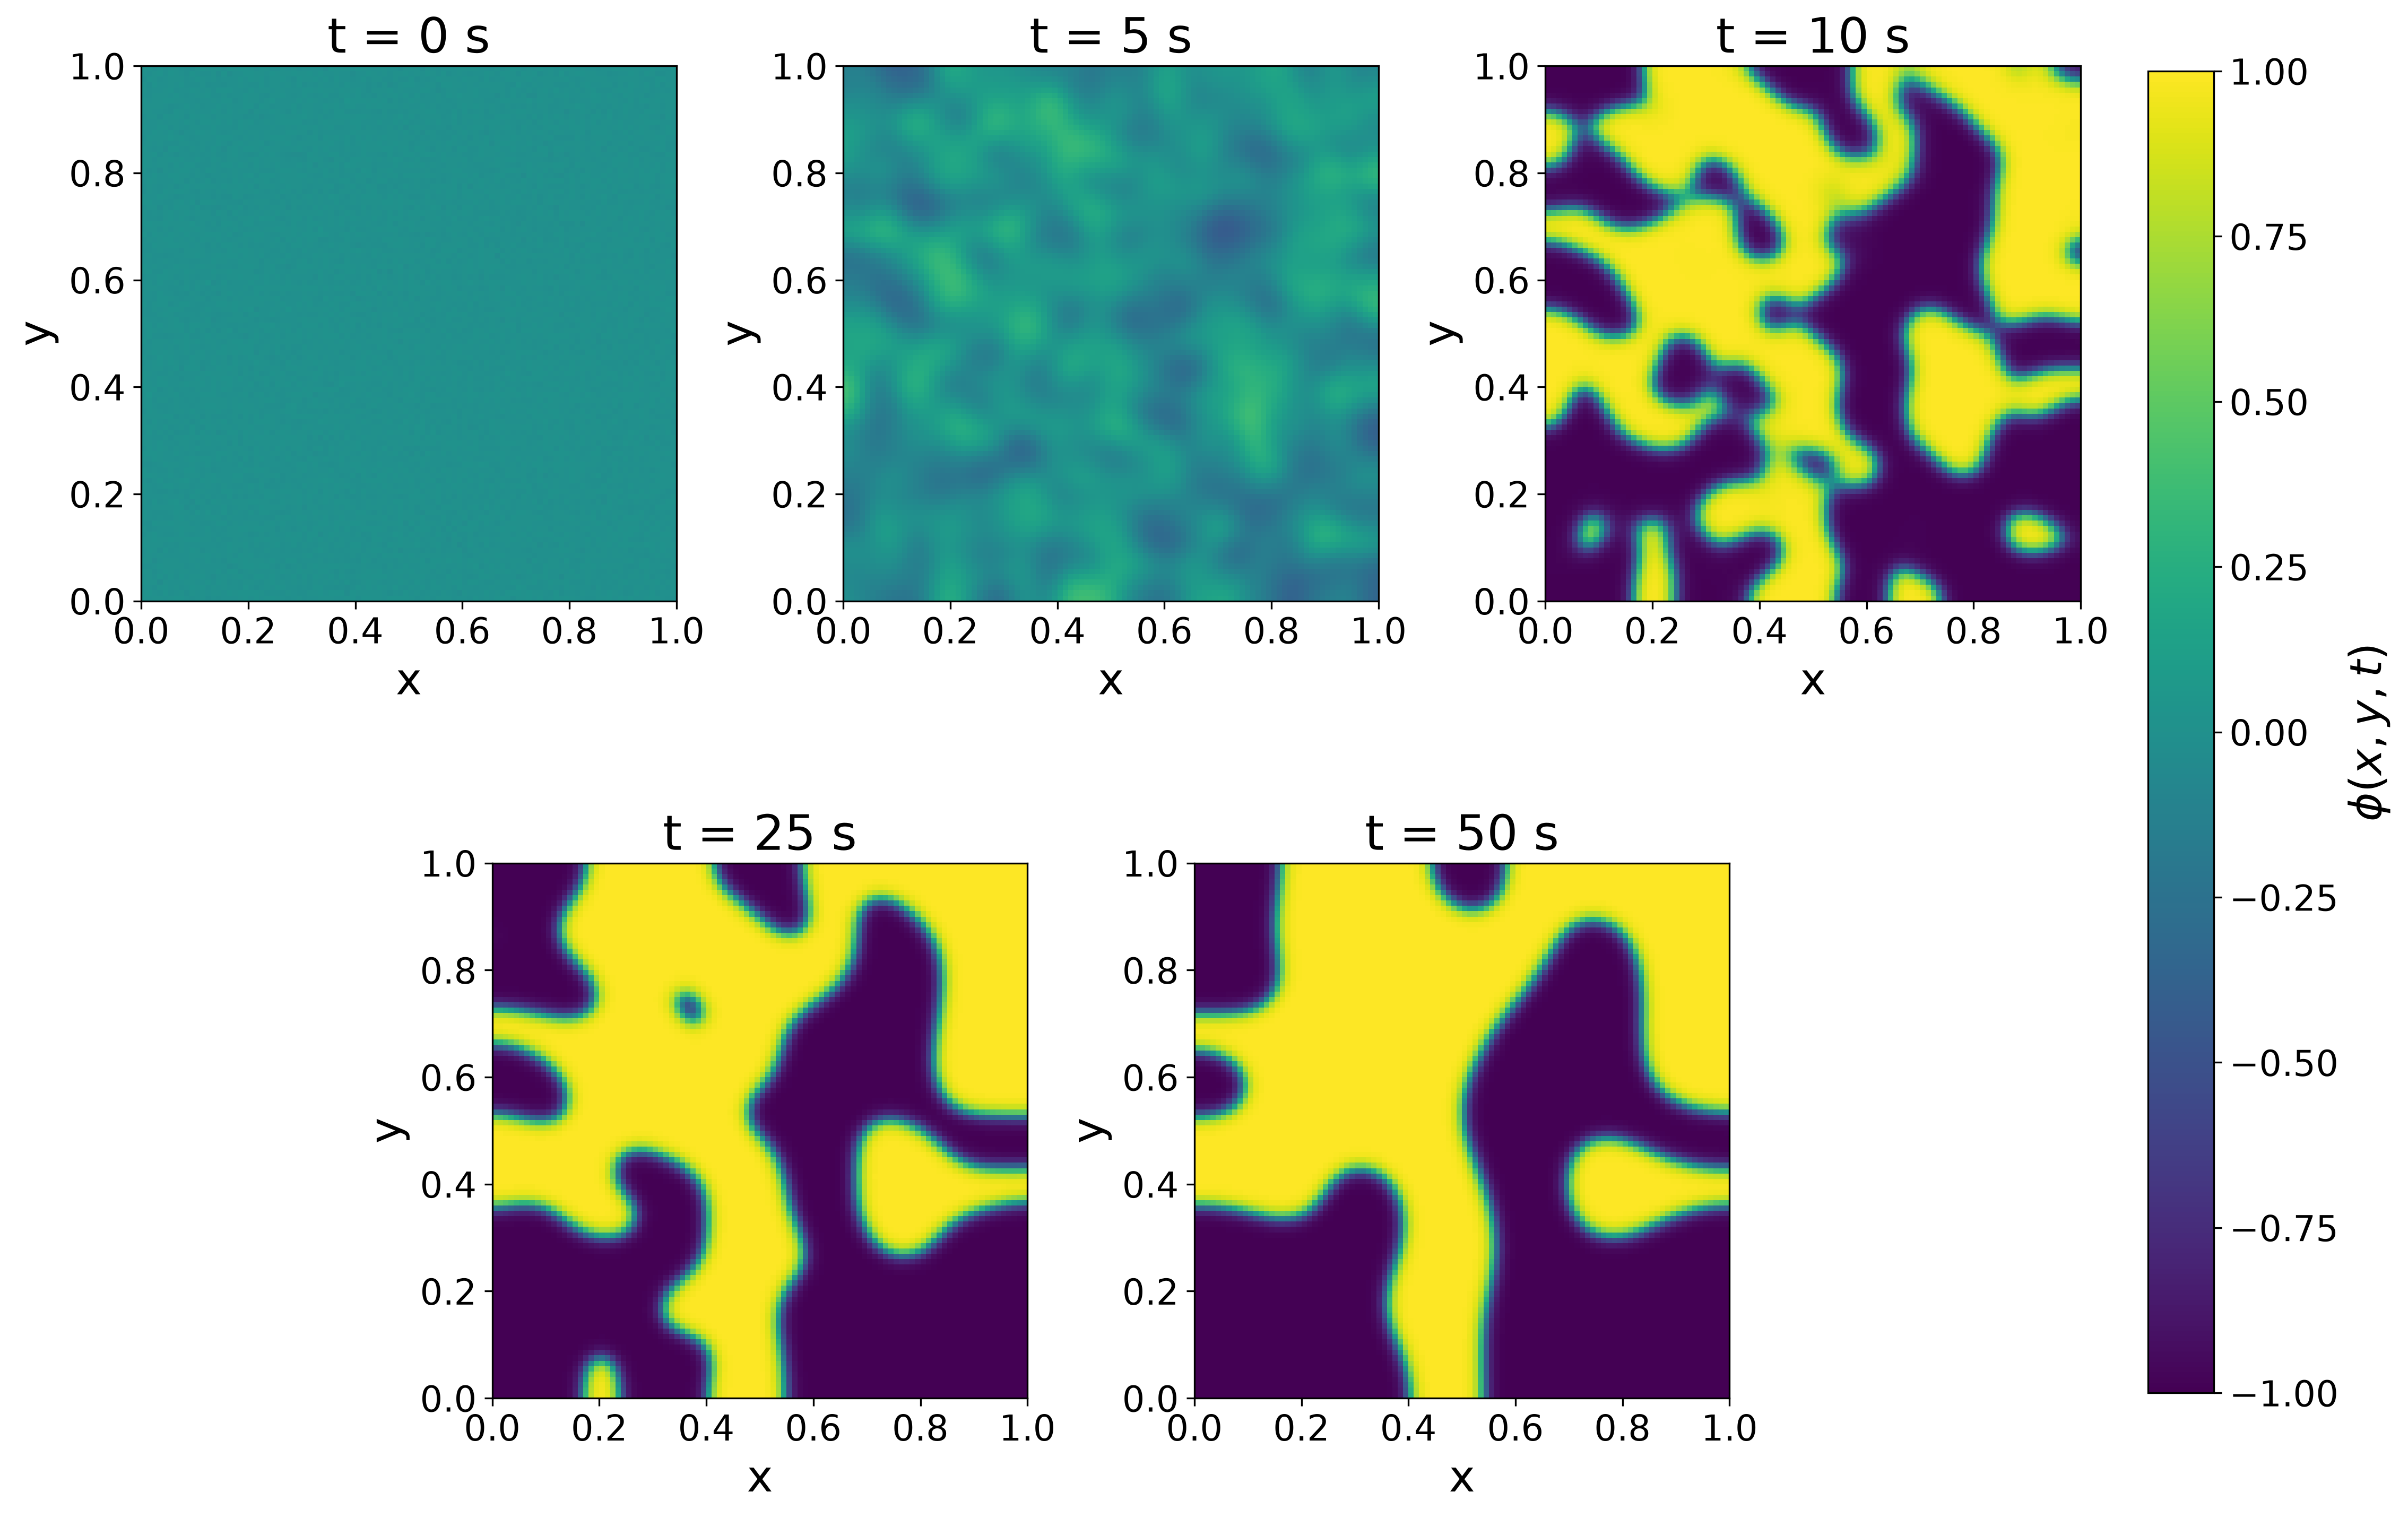
\includegraphics[width=\textwidth]
    {conservative_snapshots.png}
    \caption{Numerical solution of the conservative 
    Allen-Cahn equation at $t=0$, 5, 10, 25, and 50.}
    \label{fig:conservative_snapshots}
\end{figure}

Figure~\ref{fig:conservative_snapshots} shows that the conservative Allen-Cahn equation has similar behavior to the basic Allen-Cahn equation. The initially well-mixed fluids separate into distinct phases, and smaller regions disappear as time increases.

\begin{figure}[H]
    \centering
    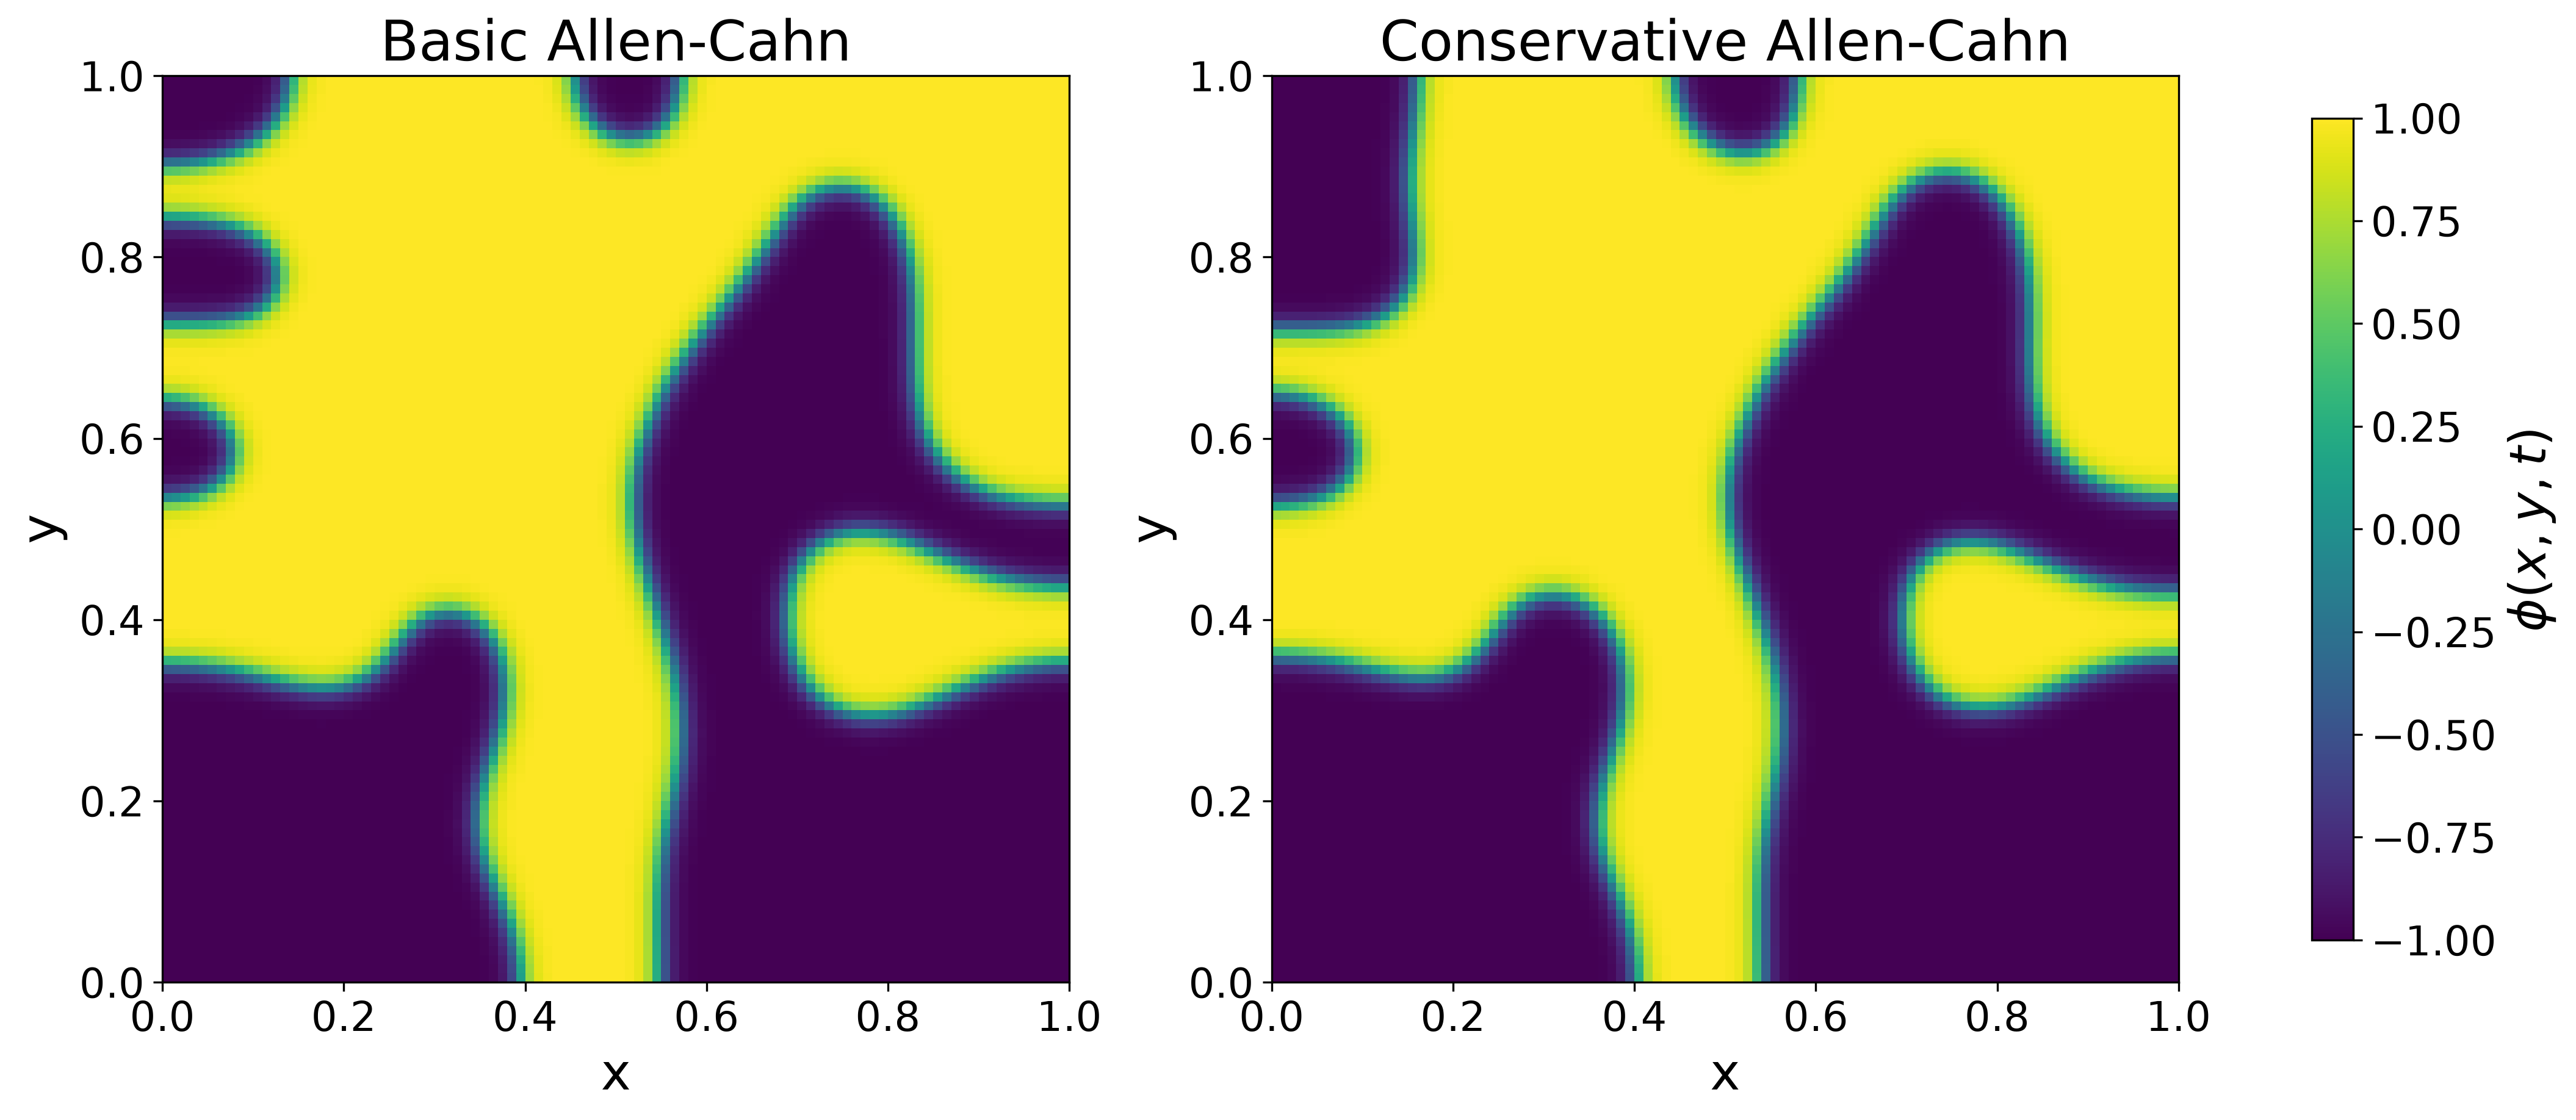
\includegraphics[width=\textwidth]
    {solution_comparison.png}
    \caption{Comparison of the basic and conservative 
    Allen-Cahn solutions at $t=50$.}
    \label{fig:solution_comparison}
\end{figure}

Figure~\ref{fig:solution_comparison} shows that the two solutions have similar overall phase distributions but differ in the locations of their interfaces. In particular, the two negative-phase regions in the upper-left corner of the basic solution have merged into one larger region in the conservative solution. \\

The conservative solution also contains a larger proportion of the negative phase than the basic solution. This makes sense because the conservative equation must maintain the initial mass, while the basic equation allows the positive phase to grow at the expense of the negative phase.

% --------------------------------------------------
\subsection*{Numerical Mass Conservation}
% --------------------------------------------------
To verify that the modified Allen-Cahn equation conserves mass, the discrete total mass was calculated at every time step:
\[
    M^n=h^2\sum_{i,j}\phi_{ij}^n.
\]

\begin{figure}[H]
    \centering
    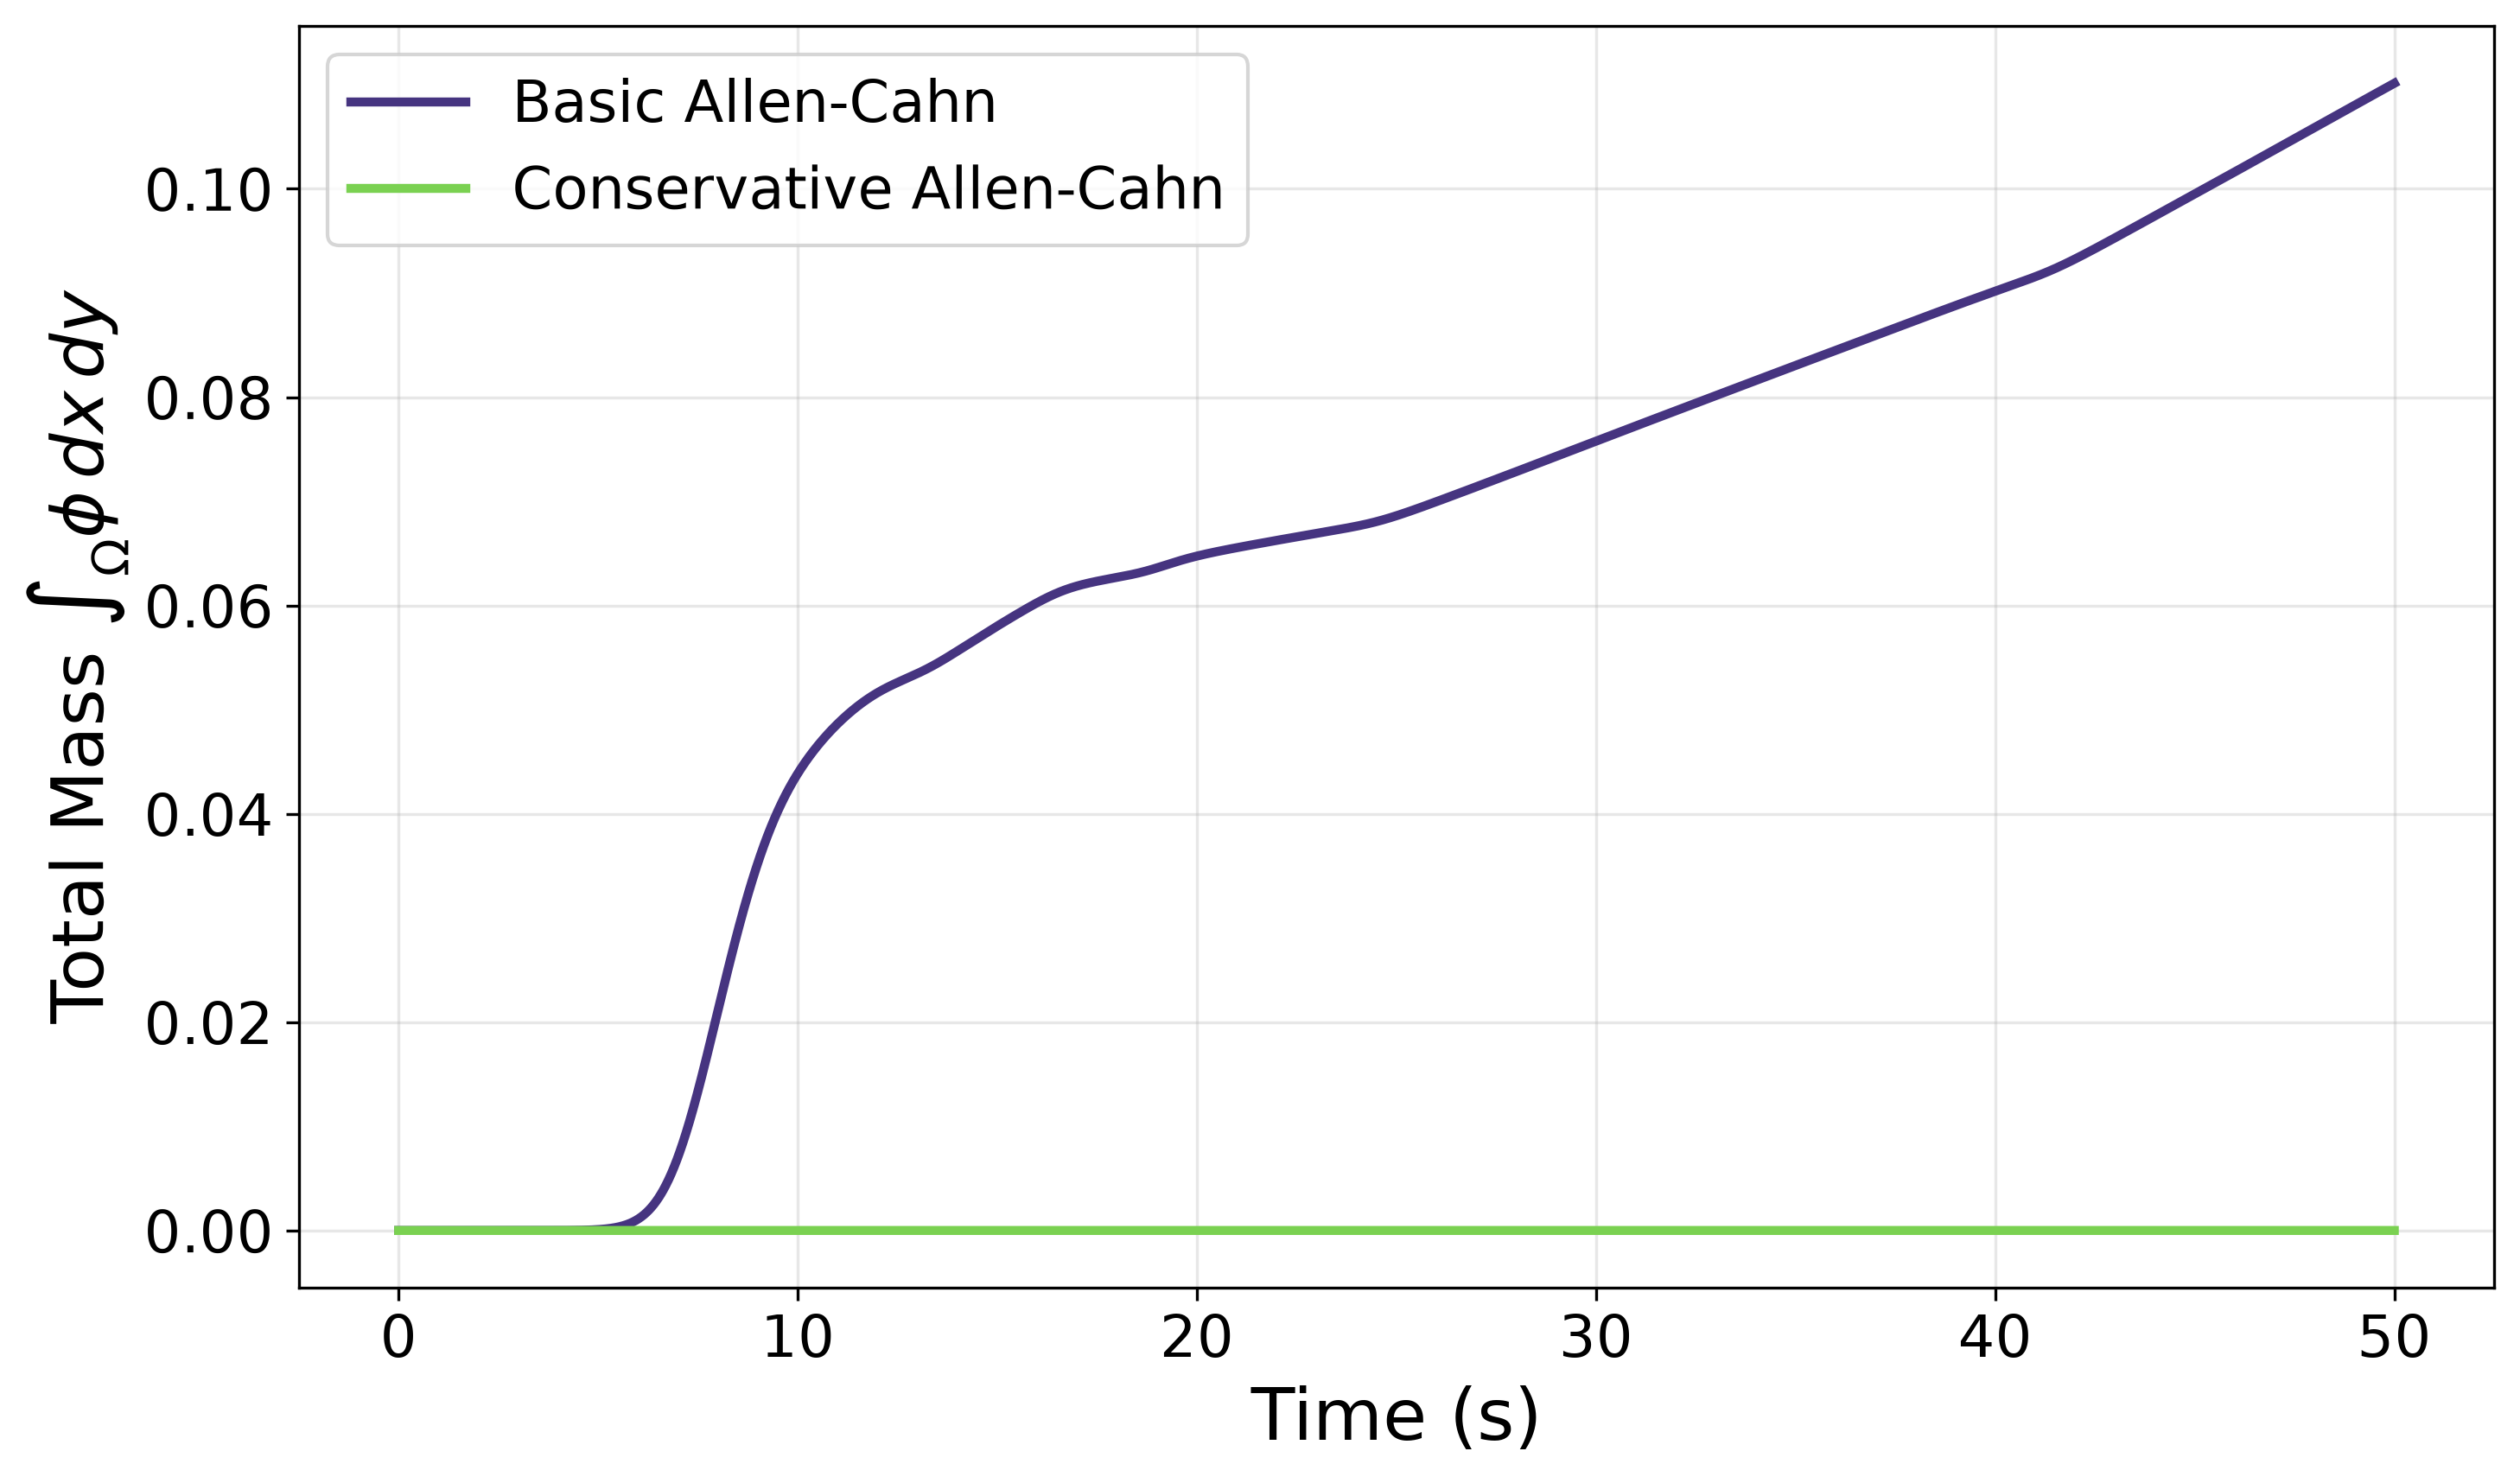
\includegraphics[width=0.9\textwidth]
    {mass_comparison.png}
    \caption{Comparison of total mass over time for 
    the basic and conservative Allen-Cahn equations.}
    \label{fig:mass_comparison}
\end{figure}

Figure~\ref{fig:mass_comparison} shows that the mass of the conservative Allen-Cahn solution remains approximately zero throughout the simulation, while the mass of the basic Allen-Cahn solution increases to approximately 0.1101. \\

I also calculated the absolute mass error at each time step:
\[
    E_{\mathrm{mass}}^n=|M^n-M^0|.
\]

The maximum mass error over the entire simulation was calculated as
\[
    E_{\mathrm{max}}
    =
    \max_n|M^n-M^0|.
\]

\begin{figure}[H]
    \centering
    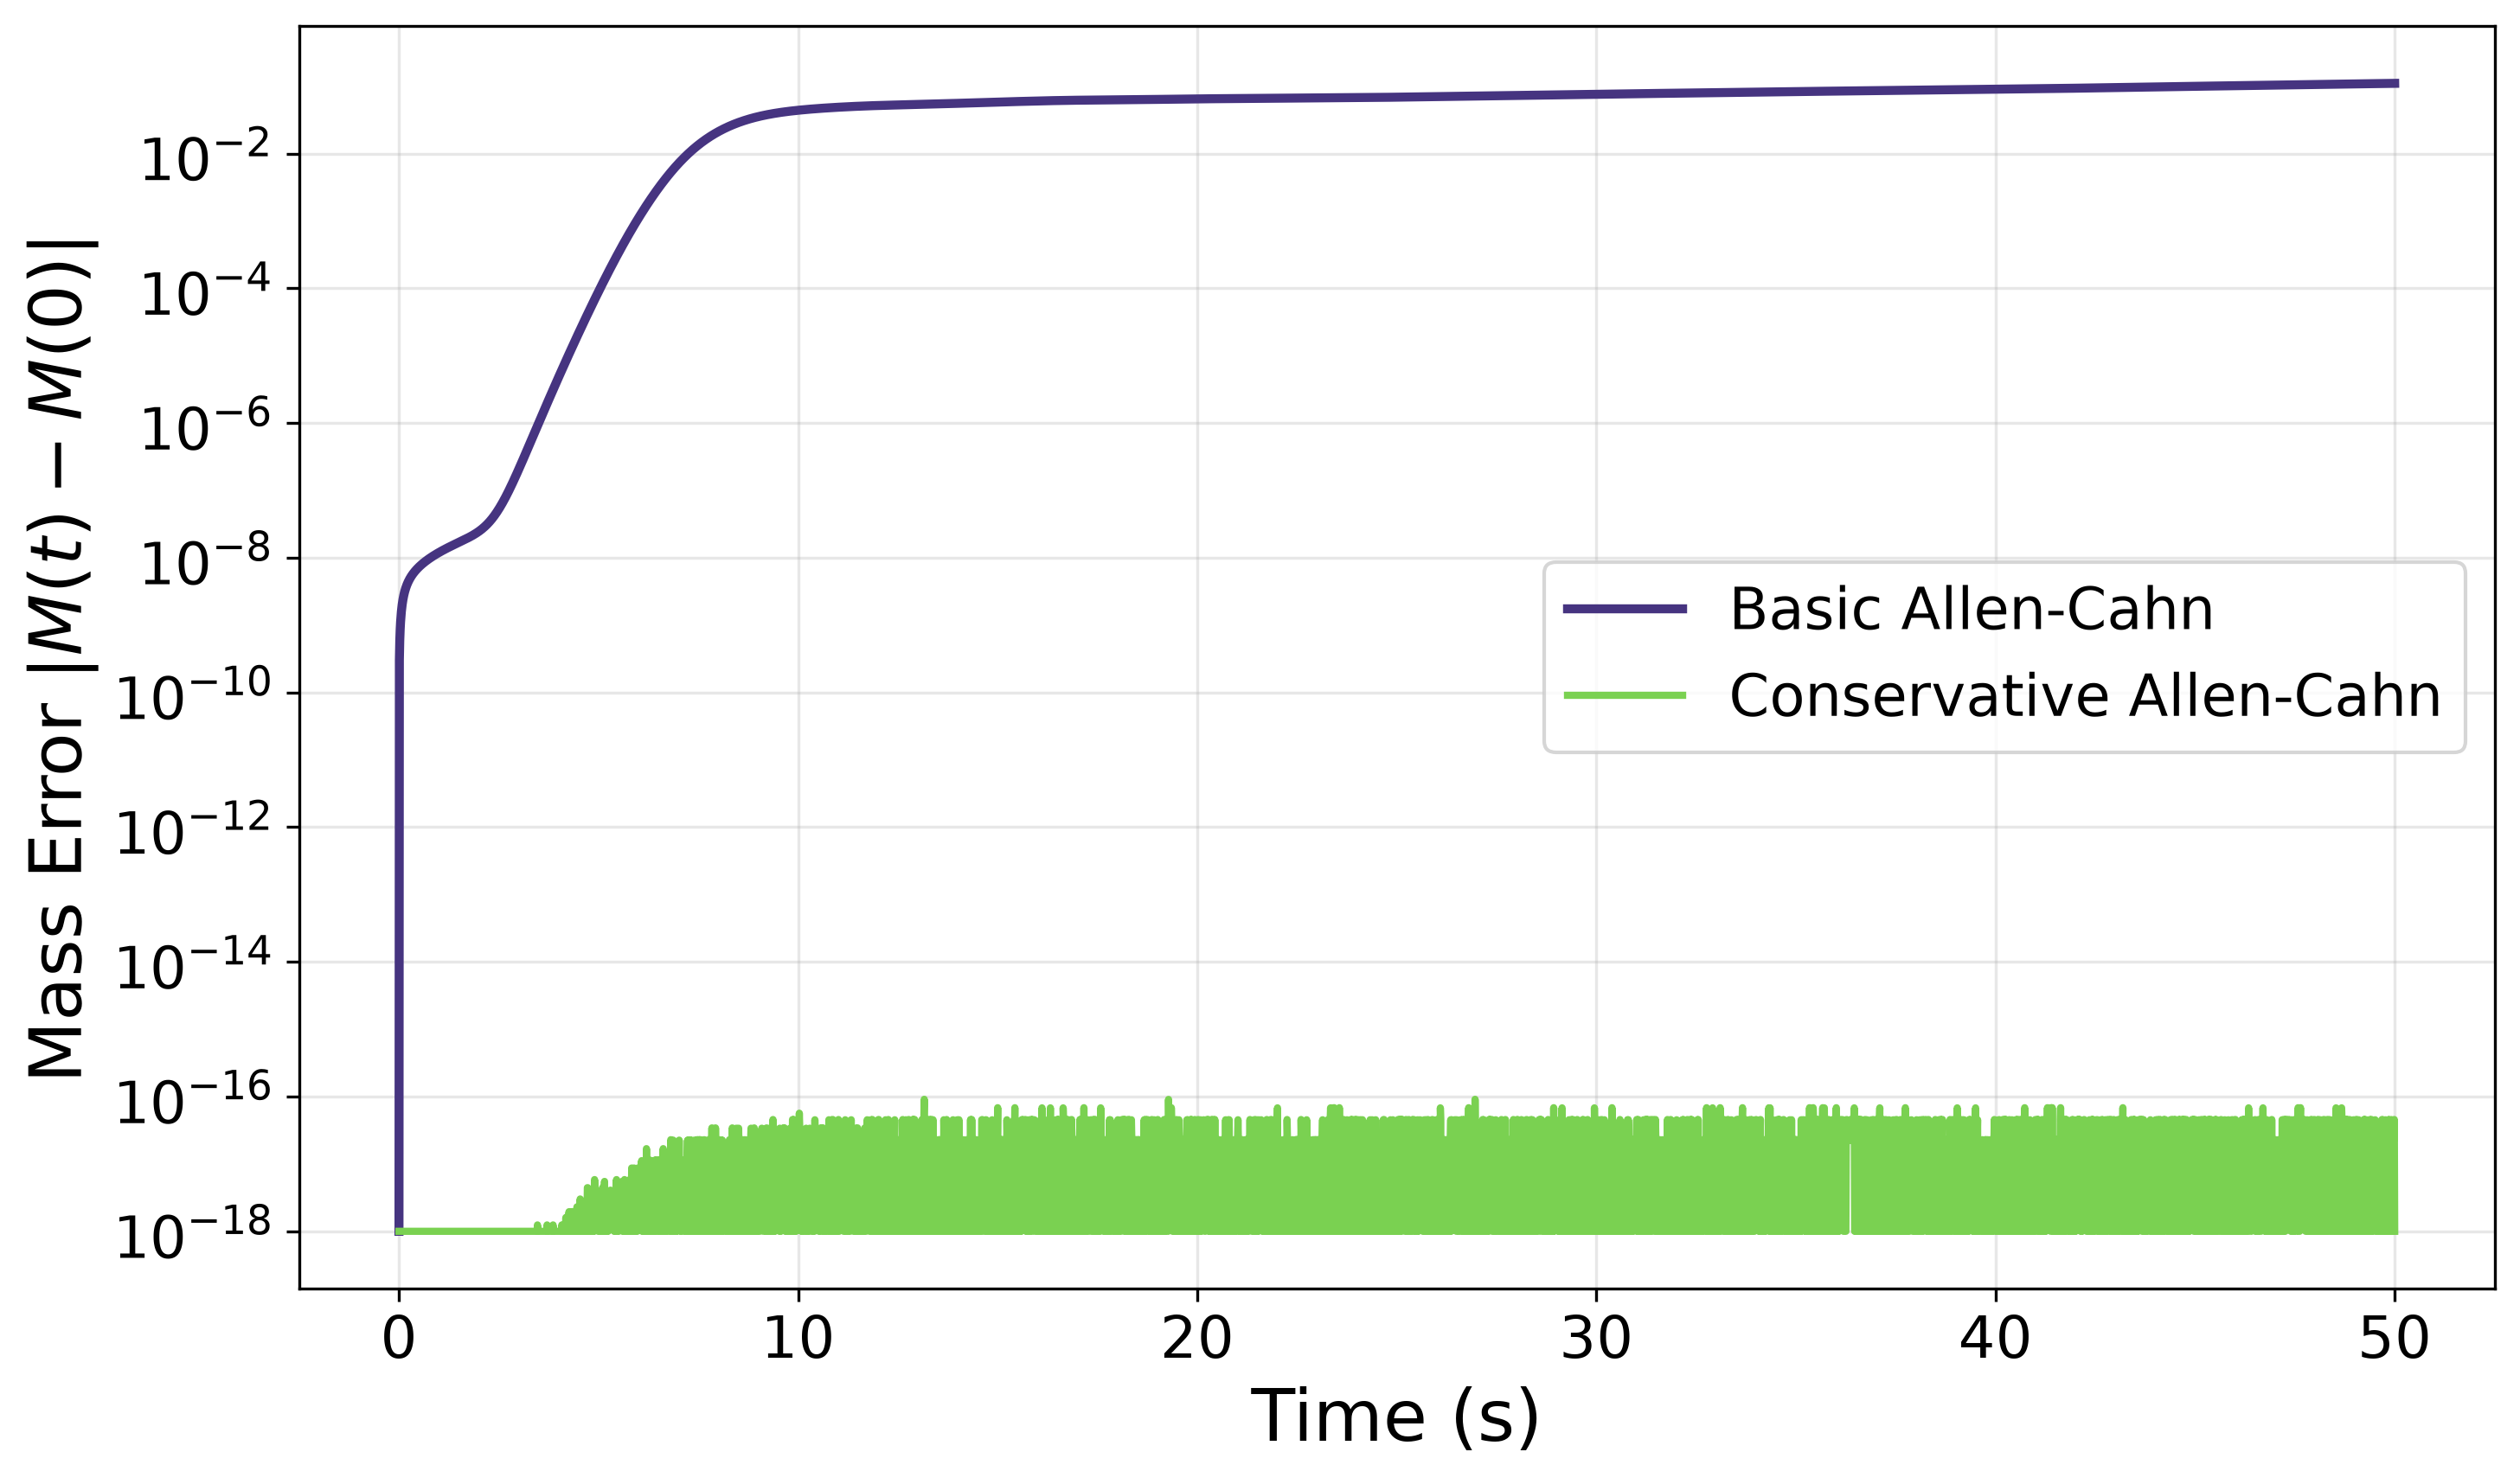
\includegraphics[width=0.9\textwidth]
    {mass_error.png}
    \caption{Absolute mass conservation error over 
    time for the basic and conservative Allen-Cahn 
    equations. A minimum plotting value of $10^{-18}$ 
    was used because zero cannot be displayed on a 
    logarithmic scale.}
    \label{fig:mass_error}
\end{figure}

Figure~\ref{fig:mass_error} shows that the mass error of the conservative Allen-Cahn equation remains below $10^{-16}$ throughout the entire simulation. The small fluctuations in the error are consistent with floating-point roundoff error.

\begin{table}[H]
    \centering
    \caption{Comparison of numerical results for the 
    basic and conservative Allen-Cahn equations.}
    \label{tab:mass_comparison}
    \begin{tabular}{|l|c|c|}
        \hline
        & Basic & Conservative \\ [0.5ex]
        \hline
        Initial Mass 
        & $-1.7764\times10^{-19}$ 
        & $-1.7764\times10^{-19}$\\
        Final Mass 
        & $1.1013\times10^{-1}$ 
        & $0$\\
        Maximum Mass Error 
        & $1.1013\times10^{-1}$ 
        & $9.1127\times10^{-17}$\\
        Minimum $\phi$ & $-1.000000$ & $-1.000000$\\
        Maximum $\phi$ & $1.000000$ & $1.000000$\\
        Runtime (s) & 4.48 & 5.08\\
        \hline
    \end{tabular}
\end{table}

Table~\ref{tab:mass_comparison} shows that the conservative Allen-Cahn equation reduces the maximum mass error by approximately 15 orders of magnitude. In other words, the operator splitting scheme conserves mass to approximately machine precision. \\

Additionally, the conservative method only required an additional 0.60 seconds of computational time. This makes sense because the mass correction only requires summations and elementwise operations rather than solving another linear system. \\

The conservative Allen-Cahn equation is therefore able to preserve the behavior of the basic equation while conserving total mass with relatively little additional computational cost.

\newpage

% ==================================================
\section*{Problem 3: Charlie's Rule}
% ==================================================
For Charlie's rule, I wanted to see what would happen if I started with fun shapes instead of randomly generated initial conditions. In other words, I wanted to see how the geometry of the initial condition would affect the solutions of the basic and conservative Allen-Cahn equations. \\

I created four different initial conditions: checkerboard, jellyfish, flower, and crescent moon. The shapes were initialized with $\phi \approx 1$ inside the shape and $\phi \approx -1$ outside the shape. For the checkerboard, the squares alternated between the two phases.

\begin{figure}[H]
    \centering
    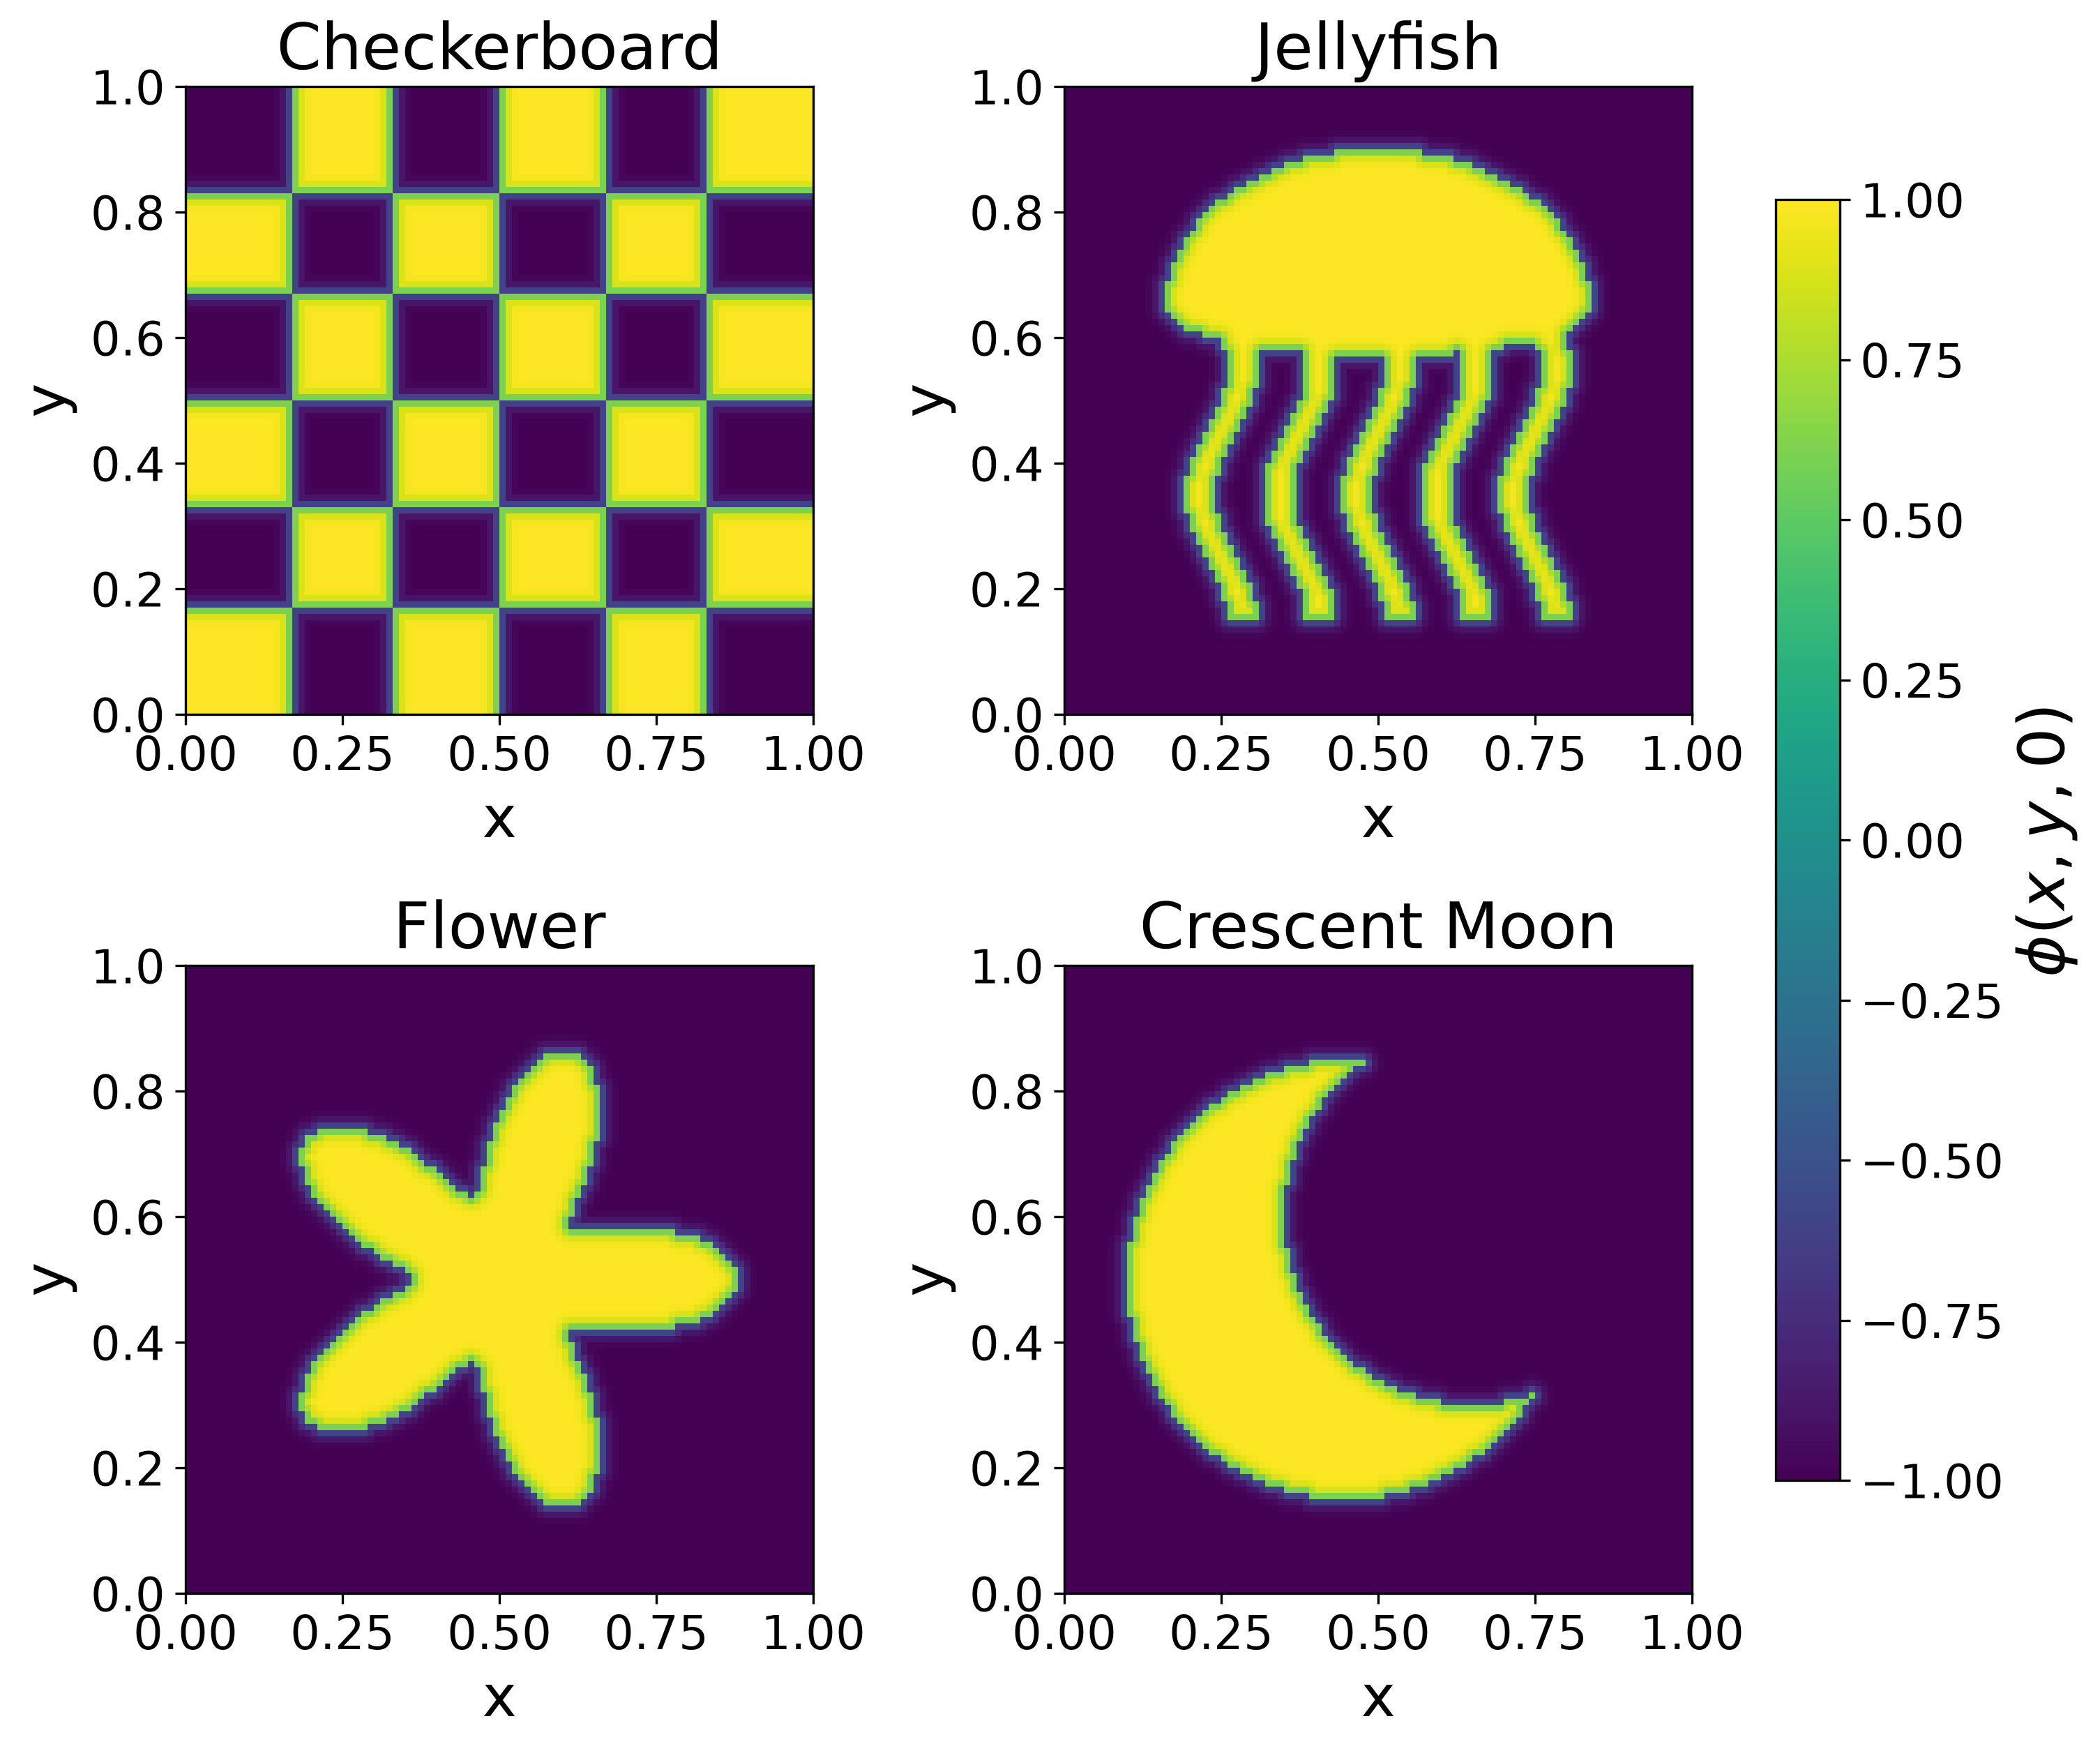
\includegraphics[width=0.95\textwidth]{charlie_initial_conditions.png}
    \caption{Four different initial conditions used to 
    explore the Allen-Cahn equations.}
    \label{fig:charlie_initial}
\end{figure}

Both equations were solved for each initial condition until $t=50$ using the same numerical methods as in Problems 1 and 2.

\begin{figure}[H]
    \centering
    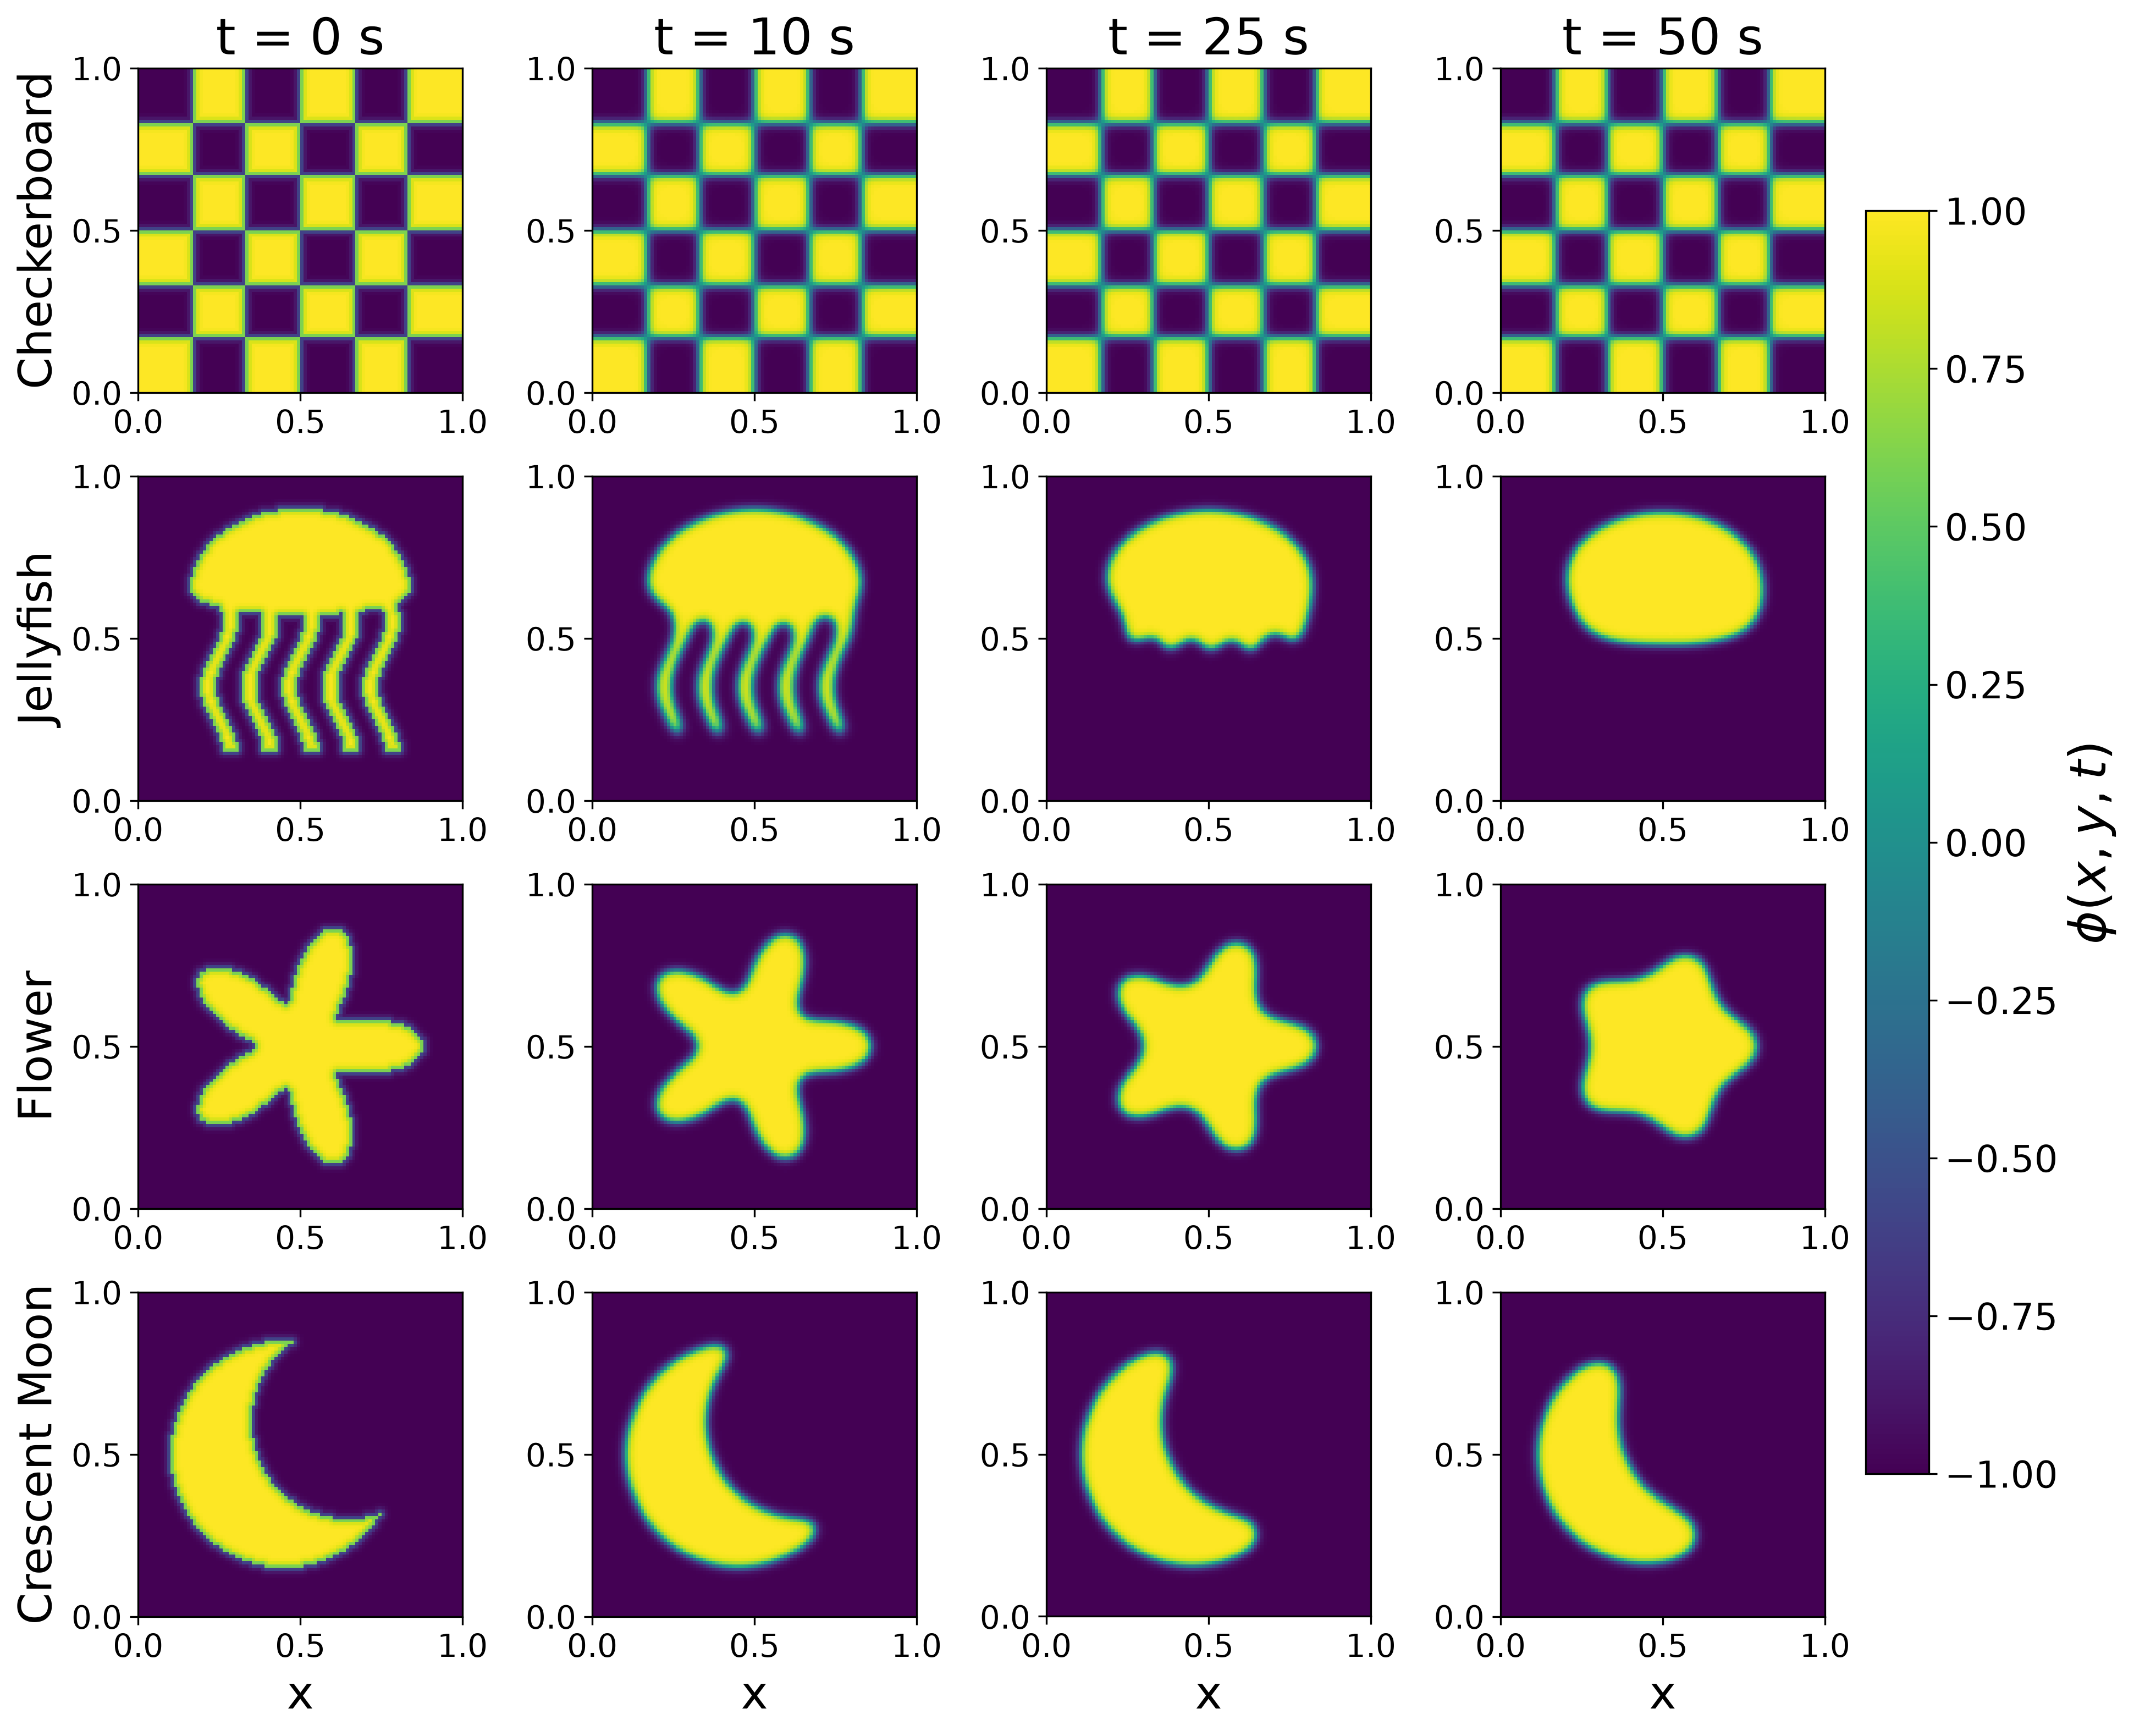
\includegraphics[width=0.95\textwidth]{charlie_basic_evolution.png}
    \caption{Evolution of the four initial conditions 
    using the basic Allen-Cahn equation.}
    \label{fig:charlie_basic}
\end{figure}

\begin{figure}[H]
    \centering
    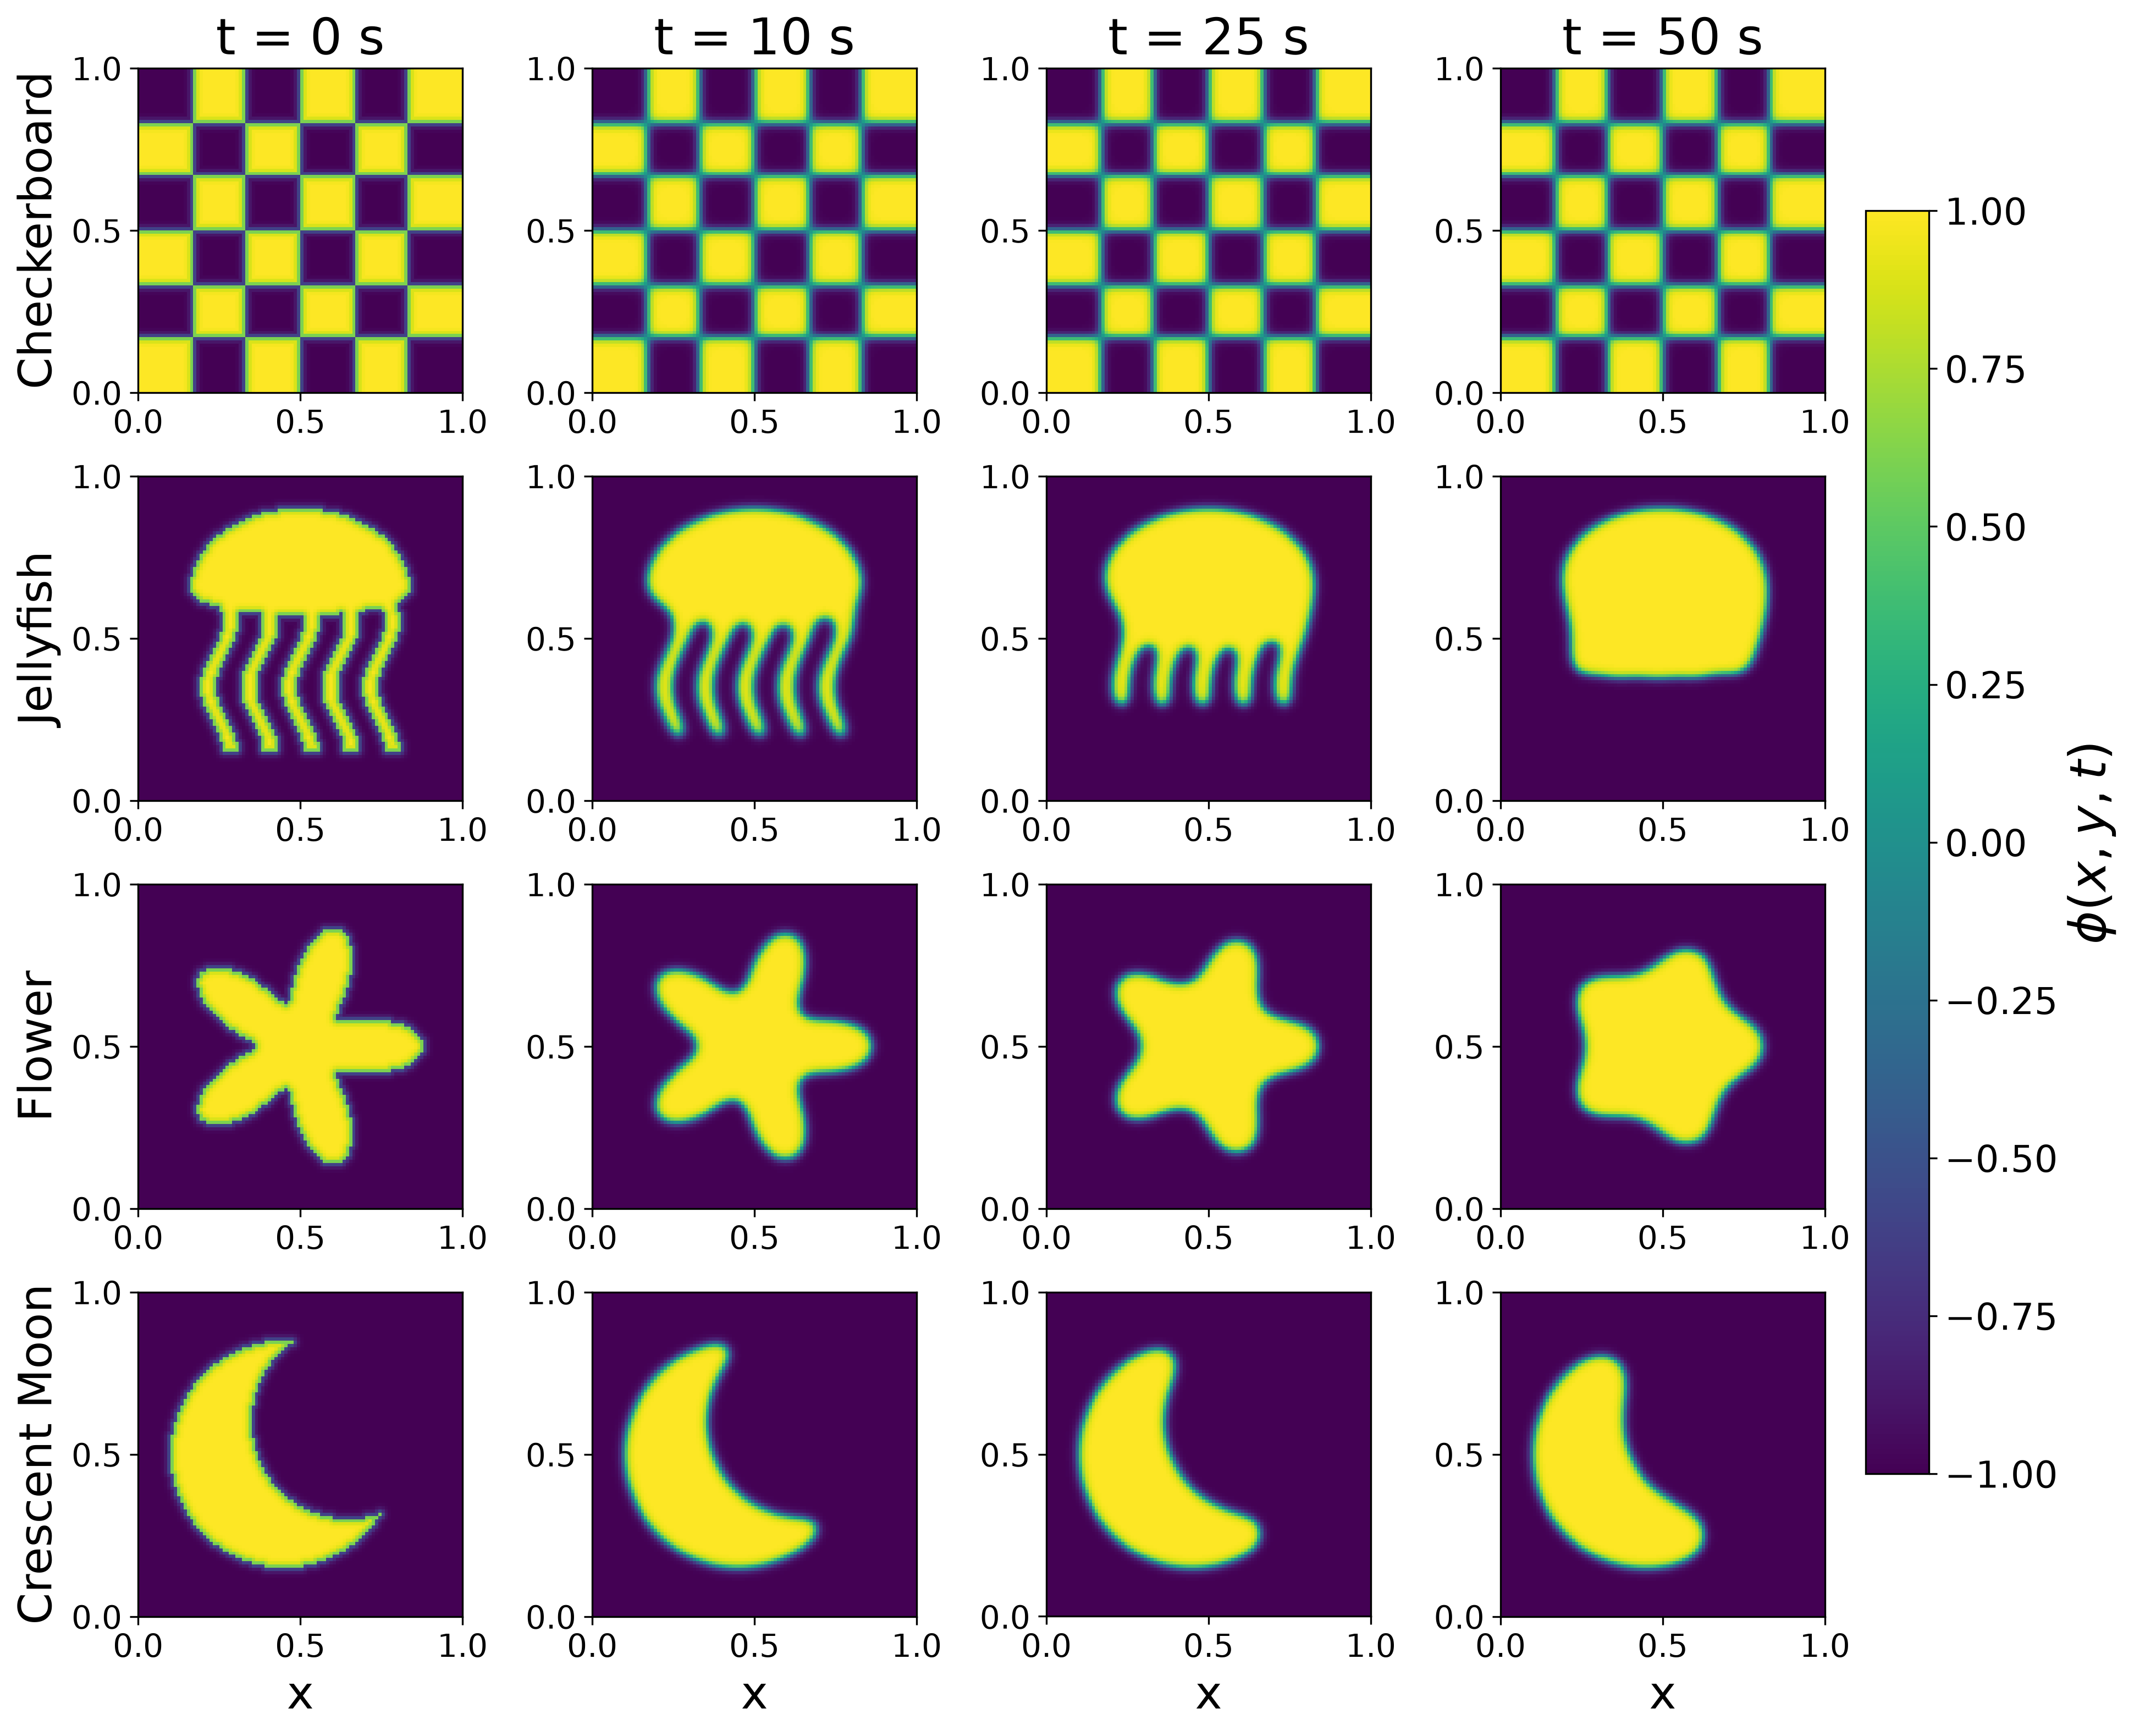
\includegraphics[width=0.95\textwidth]{charlie_conservative_evolution.png}
    \caption{Evolution of the four initial conditions 
    using the conservative Allen-Cahn equation.}
    \label{fig:charlie_conservative}
\end{figure}

Both equations smoothed out the boundaries of the shapes. The checkerboard barely changed, the flower lost some of its petal definition, and the tips of the crescent moon became more rounded. It's interesting that the jellyfish's tentacles completely disappeared by $t=50$. However, the body of the conservative jellyfish became larger to maintain its original mass. \\

I also wanted to see how well each equation preserved the total mass for the different initial conditions.

\begin{figure}[H]
    \centering
    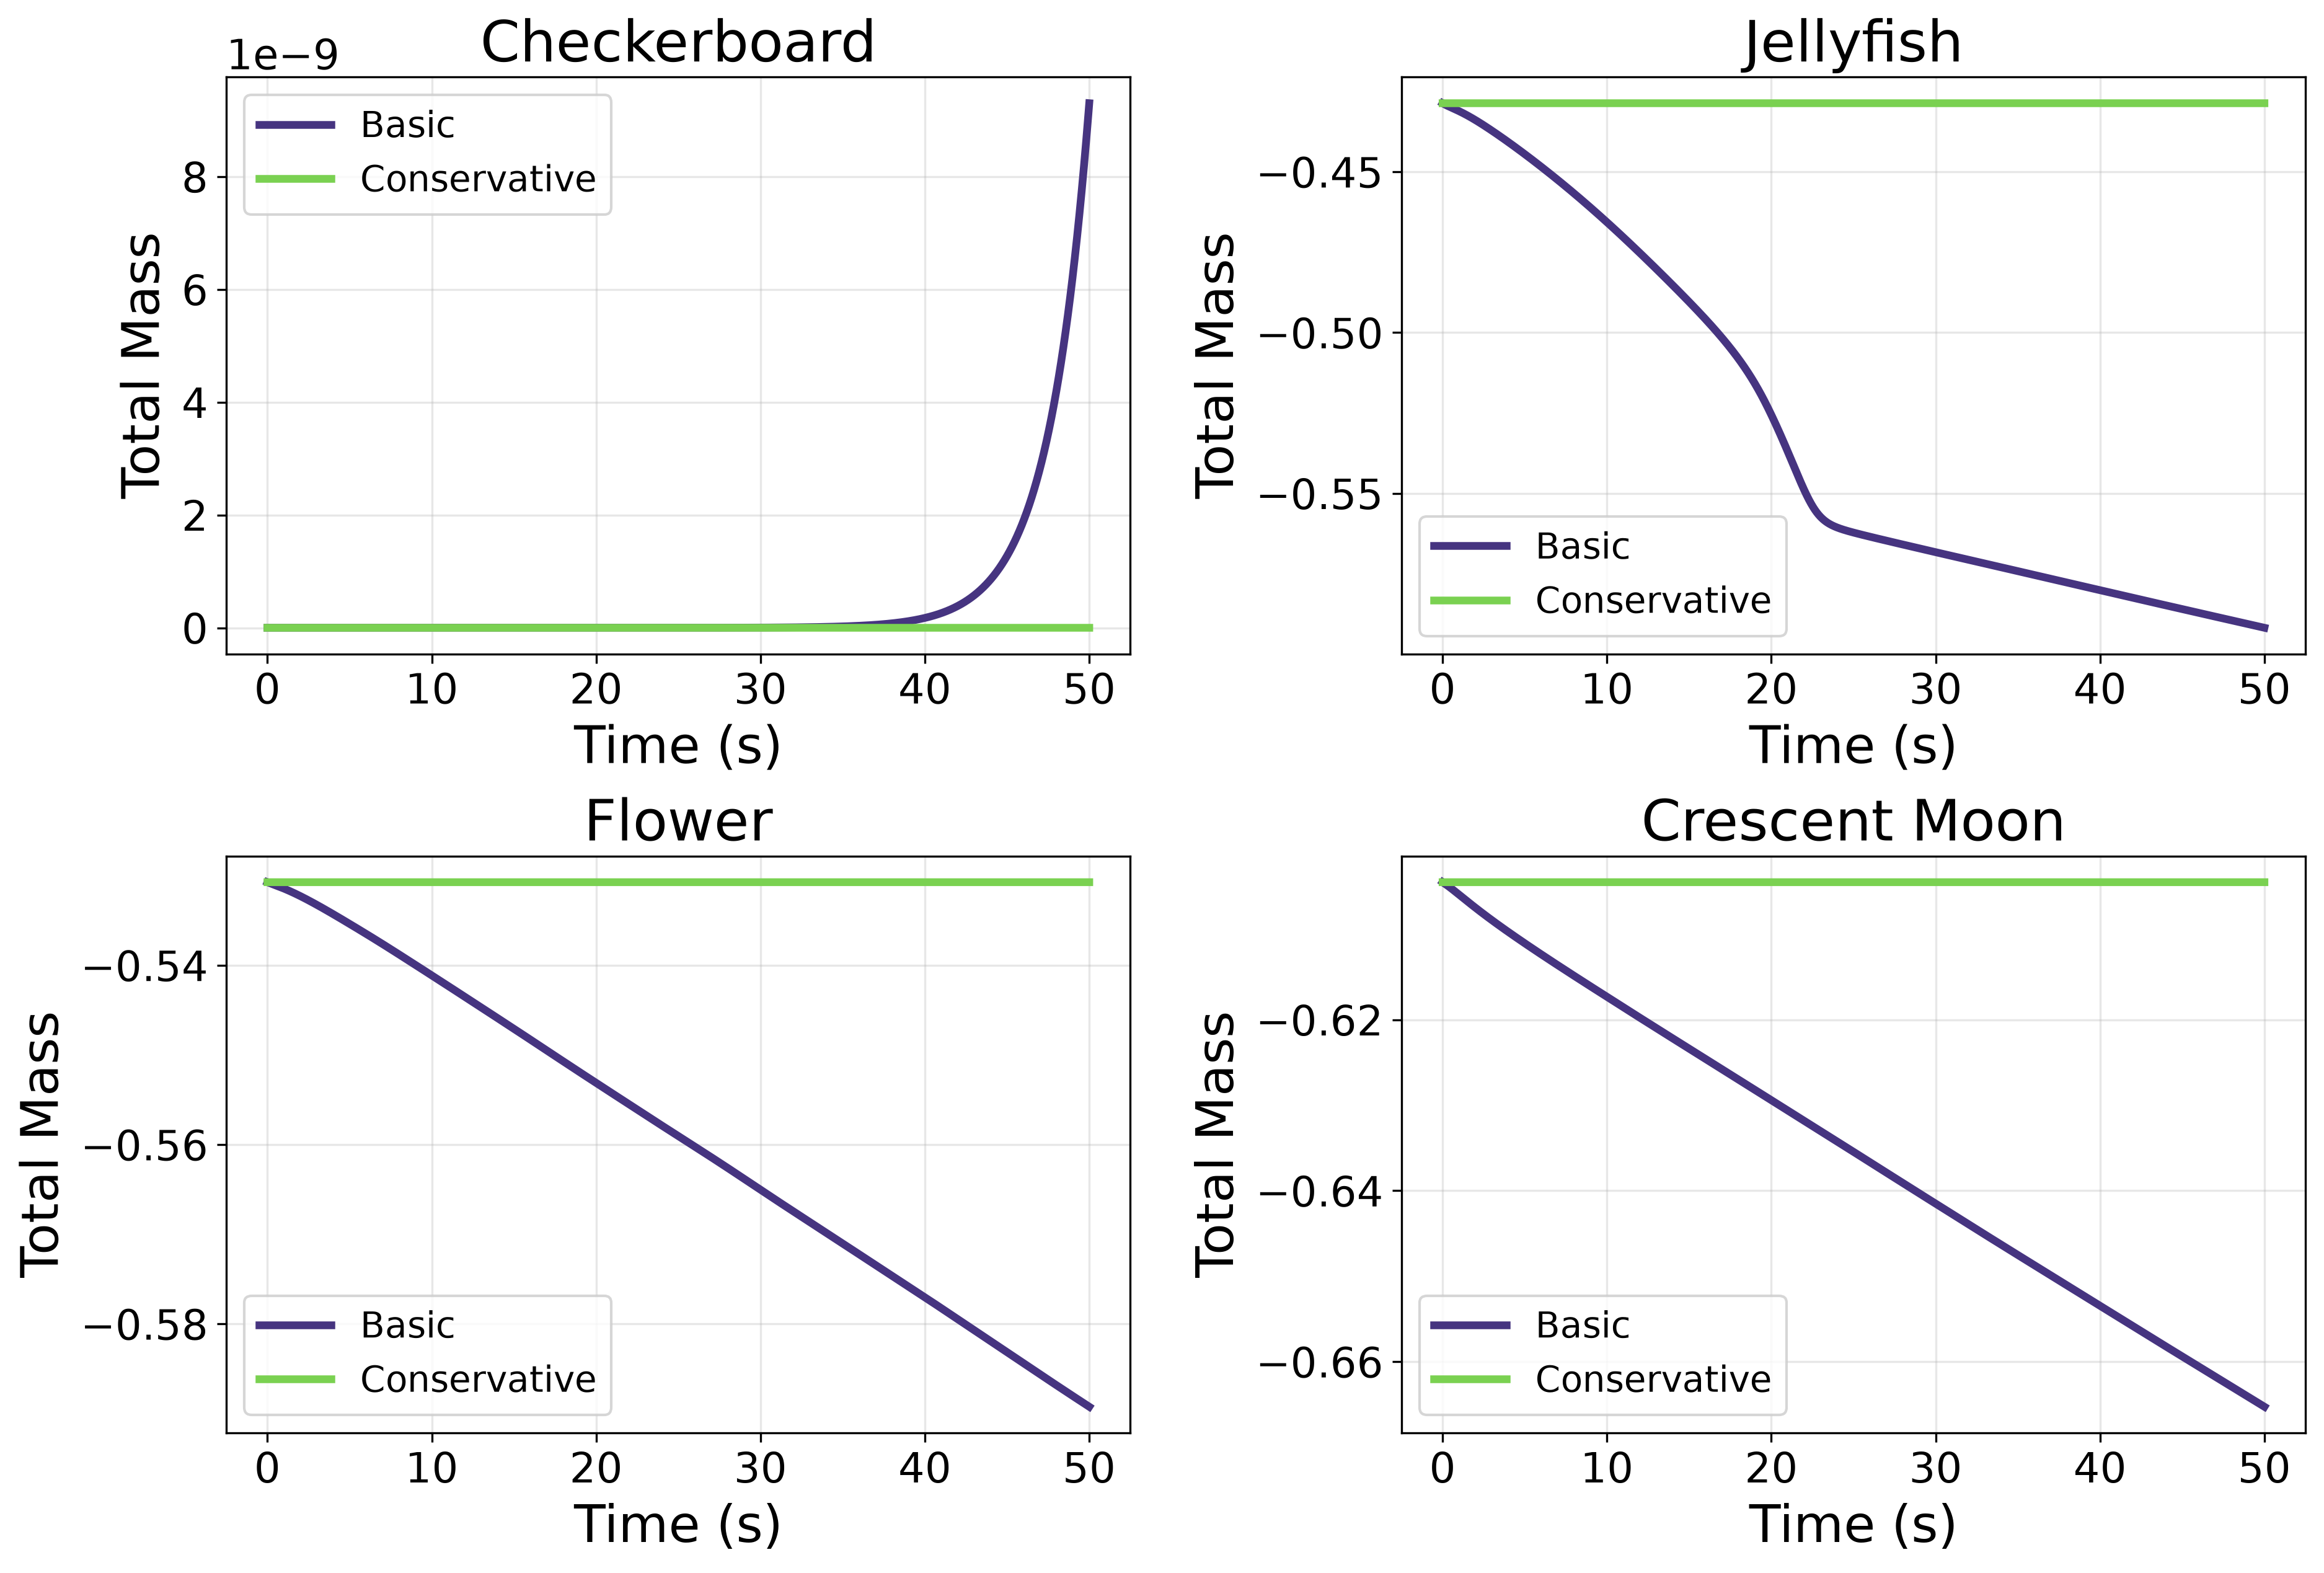
\includegraphics[width=\textwidth]{charlie_mass_comparison.png}
    \caption{Comparison of total mass over time for 
    each initial condition.}
    \label{fig:charlie_mass}
\end{figure}

The conservative equation preserved the total mass to approximately machine precision for all four initial conditions. The basic equation did not preserve mass, although the change in mass for the checkerboard was very small, likely due to its symmetry. \\

I was also interested in how much of the original shape was lost. So, I calculated the area of the positive phase by counting the grid cells where $\phi>0$:
\[
    A(t) = h^2 \sum_{i,j}
    \mathbf{1}_{\{\phi_{i,j}(t)>0\}}.
\]

The percent change in area was calculated as
\[
    \text{Area Change}
    = \frac{A(50)-A(0)}{A(0)}\times 100\%.
\]

\begin{figure}[H]
    \centering
    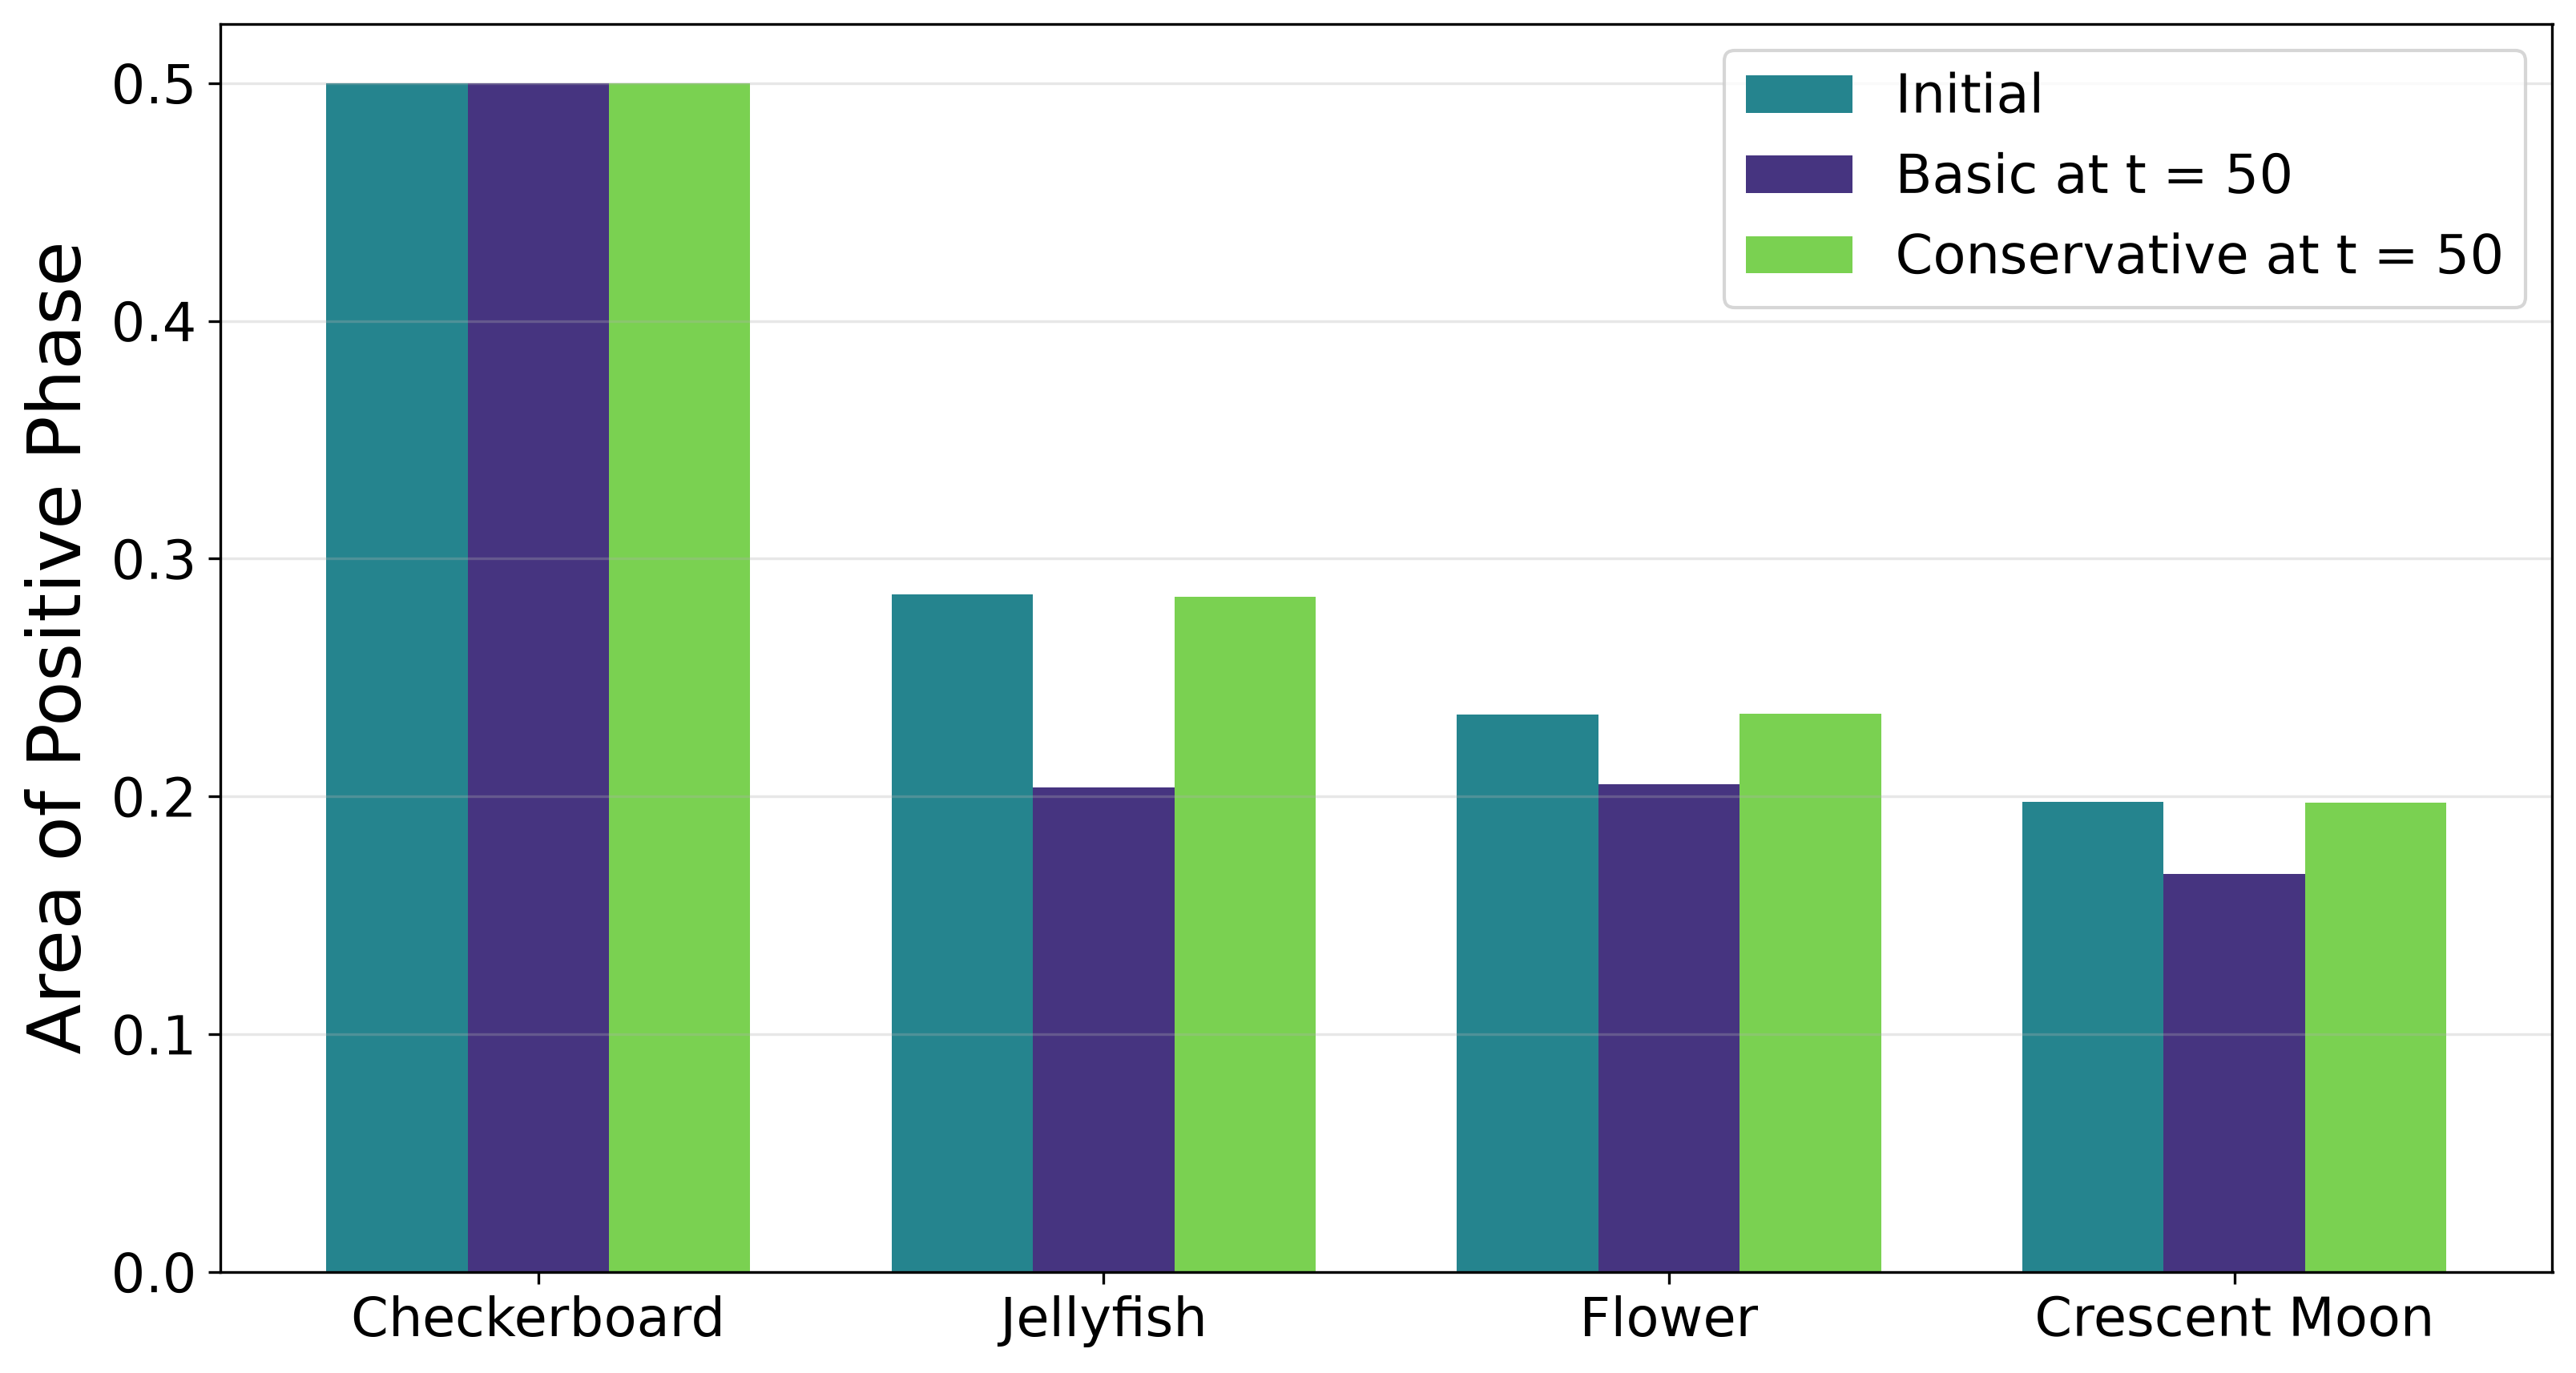
\includegraphics[width=\textwidth]{charlie_area_comparison.png}
    \caption{Initial and final positive phase areas 
    for both Allen-Cahn equations.}
    \label{fig:charlie_area}
\end{figure}

\begin{table}[H]
    \centering
    \caption{Percent change in positive phase area 
    at $t=50$.}
    \begin{tabular}{lrr}
        \toprule
        Initial Condition & Basic & Conservative \\
        \midrule
        Checkerboard  & 0.00\%   & 0.00\%  \\
        Jellyfish     & -28.41\% & -0.28\% \\
        Flower        & -12.54\% & 0.17\%  \\
        Crescent Moon & -15.33\% & -0.10\% \\
        \bottomrule
    \end{tabular}
    \label{tab:charlie_area}
\end{table}

The jellyfish had the largest decrease in area for the basic equation, losing 28.41\% of its original area. Meanwhile, the conservative equation maintained the original area of every shape to within 0.28\%. I think the area is not exactly conserved because we are conserving the integral of $\phi$ rather than the area where $\phi>0$. \\


\end{document}